%%%%%%%%%%%%%%%%%%%%%%%%%%%%%%%%%%%%%%%%
% basic elements

\documentclass[12pt]{article}
\usepackage[english]{babel}
\usepackage{amsmath,amsthm}
\usepackage{amsfonts}
\usepackage{makecell}
\usepackage{graphics}
\usepackage{graphicx}
\usepackage{fancyhdr}
\usepackage{ifthen}
\usepackage{wrapfig}
\usepackage{array}
\usepackage{colortbl}
\usepackage{fullpage}
\usepackage[table]{xcolor}
\usepackage{subfigure}
\usepackage{caption}
\usepackage{float}
\usepackage{ctex}
\usepackage{appendix}
\usepackage{shorttoc}
\usepackage{pagenote}
\usepackage{setspace}
\usepackage{geometry}
\usepackage{indentfirst}
\usepackage{fullpage}
\usepackage{booktabs}
\usepackage{multirow}
\usepackage{longtable}
\usepackage{minipage-marginpar}
\usepackage{hyperref}
\usepackage{palatino}
\usepackage{setspace}
\usepackage{subfigure}
\usepackage{picinpar}
\usepackage{newtxtext}
\usepackage{amsmath,amssymb,amsthm}
\usepackage{newtxmath} % must come after amsXXX

% Replace ABCDEF in the next line with your chosen problem
% and replace 111111 with your Team Control Number
% and replace abcdef with your Title
% and replace 123456 with the number of pages of your essay
\newcommand{\Problem}{B}
\newcommand{\Team}{{12003}}
\newcommand{\Title}{{Tackling the Drought}}
\newcommand{\wholepages}{21}
\title{\huge\textbf{Tackling the Drought}}
\author{Team\#\Team}
\date{\today}

%%%%%%%%%%%%%%%%%%%%%%%%%%%%%%%%%%%%%%%%
% set up of theorems

\newtheorem{thm}{Theorem}[section]
\newtheorem{cor}[thm]{Corollary}
\newtheorem{lem}[thm]{Lemma}
\newtheorem{prop}[thm]{Proposition}
\theoremstyle{definition}
\newtheorem{defn}[thm]{Definition}
\theoremstyle{remark}
\newtheorem{rem}[thm]{Remark}
\numberwithin{equation}{section}
\newtheorem{theorem}{Theorem}
\newtheorem{corollary}[theorem]{Corollary}
\newtheorem{lemma}[theorem]{Lemma}
\newtheorem{definition}{Definition}

%%%%%%%%%%%%%%%%%%%%%%%%%%%%%%%%%%%%%%%%
% setup of page length and script size

\setlength{\belowcaptionskip}{9pt}
\setlength{\abovecaptionskip}{9pt}
\setlength{\headsep}{0.4in}
\setlength{\headheight}{14.5pt}
\captionsetup{font={footnotesize}}
\renewcommand{\baselinestretch}{1.1}
\geometry{bottom=1in}

%%%%%%%%%%%%%%%%%%%%%%%%%%%%%%%%%%%%%%%%
% set up of page style

\pagestyle{fancy}
\fancyhead[L]{Team\ \#\Team}
\fancyhead[C]{\Title}
\fancyhead[R]{Page \thepage \ of \wholepages}
\fancyfoot{}

%%%%%%%%%%%%%%%%%%%%%%%%%%%%%%%%%%%%%%%%
% hyphenation

\tolerance=1
\emergencystretch=\maxdimen
\hyphenpenalty=10000
\hbadness=10000

\hypersetup{hidelinks} 
\hypersetup{
	colorlinks=false,
	linkcolor=black,
	citecolor=black,
	anchorcolor=black
}

%%%%%%%%%%%%%%%%%%%%%%%%%%%%%%%%%%%%%%%%
% biblography
\bibliographystyle{plain}
% \usepackage{url}
% \def\UrlBreaks{\do\A\do\B\do\C\do\D\do\E\do\F\do\G\do\H\do\I\do\J\do\K\do\L\do\M\do\N\do\O\do\P\do\Q\do\R\do\S\do\T\do\U\do\V\do\W\do\X\do\Y\do\Z\do\[\do\\\do\]\do\^\do\_\do\`\do\a\do\b\do\c\do\d\do\e\do\f\do\g\do\h\do\i\do\j\do\k\do\l\do\m\do\n\do\o\do\p\do\q\do\r\do\s\do\t\do\u\do\v\do\w\do\x\do\y\do\z\do\.\do\@\do\\\do\/\do\!\do\_\do\|\do\;\do\>\do\]\do\)\do\,\do\?\do\'\do+\do\=\do\#}

%%%%%%%%%%%%%%%%%%%%%%%%%%%%%%%%%%%%%%%%
% end of the beginning part
\begin{document}
	\DeclareGraphicsExtensions{.pdf, .jpg, .tif, .png}
	\thispagestyle{empty}
	\vspace*{-16ex}
	% MCM/ICM Template
	% \centerline{\begin{tabular}{*3{c}}
			%	\parbox[t]{0.3\linewidth}{\begin{center}\textbf{Problem Chosen}\\ \Large \Problem\end{center}}
			%	& \parbox[t]{0.3\linewidth}{\begin{center}\textbf{2020\\ MCM \\ Summary Sheet}\end{center}}
			%	& \parbox[t]{0.3\linewidth}{\begin{center}\textbf{Team Control Number}\\ \Large Team \# \Team\end{center}}	\\
			%	\hline
			%\end{tabular}}
	% HiMCM/IMMC Template
	\begin{center}
		\centerline{\begin{tabular}{p{\linewidth}<{\centering}}
				\small Team Control Number \\
				\huge \textbf{\Team} \\
				\small Problem Chosen \\
				\huge \textbf{\Problem} \\
				\textbf{2021} \\
				\small \textbf{HiMCM / MidMCM} \\
				\small \textbf{Summary Sheet} \\
				\hline
		\end{tabular}}
	\end{center}
%%%%%%%%%%% Begin Summary %%%%%%%%%%%%%%%%%%
% Enter your summary here replacing the (red) text
% Replace the text from here ...
\qquad
\par

In the summer of 2021, Lake Mead, a part of the Colorado River and the largest water reservoir in the US, announced water shortage due to drought caused by climate change. With the aggravation of climate change, water shortage has exerted a negative impact on the agricultural regions and water delivery nearby, so finding a way to solve this problem is of much importance. Our goal was to create models which can analyze drought impact on water reservoirs based on the example of Lake Mead as well as purpose a plan using wastewater recycling technology.

Firstly, the origins and the flowing conditions of Lake Mead were analyzed, including its inflow, other sources and its outflow. We considered the factors posing an impact on Lake Mead and raised formulas describing the relationship between them.

Next, we made a model of the spatial structure of Lake Mead. Formulas for the relationship between Volume - Area and Area - Depth are raised and tested using the data provided.

After that, several charts were plotted from water level of Lake Mead from 1935 to 2021 and we focused on its rise and fall, especially when it comes to drought period. By finding the patterns from these charts, we made some criteria for the drought periods and its factors such as beginning and end.

In addition, prediction are made for the future water levels of Lake Mead by data from the recent drought. Linear fit was used within three cycles, and the change in gradient and intercept are assumed as continuing in the same cycle in the future. Therefore, data for 2025, 2030 and 2050 was calculated.

Furthermore, we used the formulas in the first and second part and solved them to describe the water level more scientifically. Differential equations are solved and the constants are fitted using the given data from 2005 to 2021. Considering the average constant, data for the future are calculated, which has only little difference between the fit model.

Last but not least, we considered the impact of the change in water level to nearby residents, and considered the plan of building a sewage plant. Both scientific issues and government issues are taken into consideration, which resulted in two possible outcomes of the location of the sewage plant.

% to here
%%%%%%%%%%% End Summary %%%%%%%%%%%%%%%%%%%
\thispagestyle{empty}
\maketitle
\thispagestyle{empty}
\newpage
%%%%%%%%%%%%%%%%%%%%%%%%%%%%%%%%%%%%%%%%
\clearpage
\thispagestyle{empty}
% Uncomment the next line to generate a Table of Contentsr%r%\shortableofcontents{Contents}{2}
\tableofcontents % Uncomment this line to update the Contents
\newpage
\pagestyle{fancy}
\setcounter{page}{1}
% Begin your paper here
%%%%%%%%%%%%%%%%%%%%%%%%%%%%%%%%%%%%%%%%

\newpage
\section{Introduction}

	\subsection{Background}
	Lake Mead is a reservoir formed by the Hoover Dam on the Colorado River in the Southwestern United States. It is located in Nevada and Arizona, 24 miles east from the Las Vegas Strip. In terms of water volume, it is the largest reservoir in the United States. Built on September 30, 1935 by the Hoover Dam, the reservoir provides water to Arizona, California, Nevada, and some states in Mexico to provide livelihoods of nearly 20 million people and large areas of farmland. It plays a role in agricultural development and the daily lives of people in nearby areas.

	Since 1983, due to drought and increased water volume, the lake has been below full capacity. This essay will analyze the historical elevation patterns and predict future water levels, as well as find an energy-effecient and money-saving plan which will impose the greatest effect on the lake. \cite{Lake Mead}


		\begin{center}
		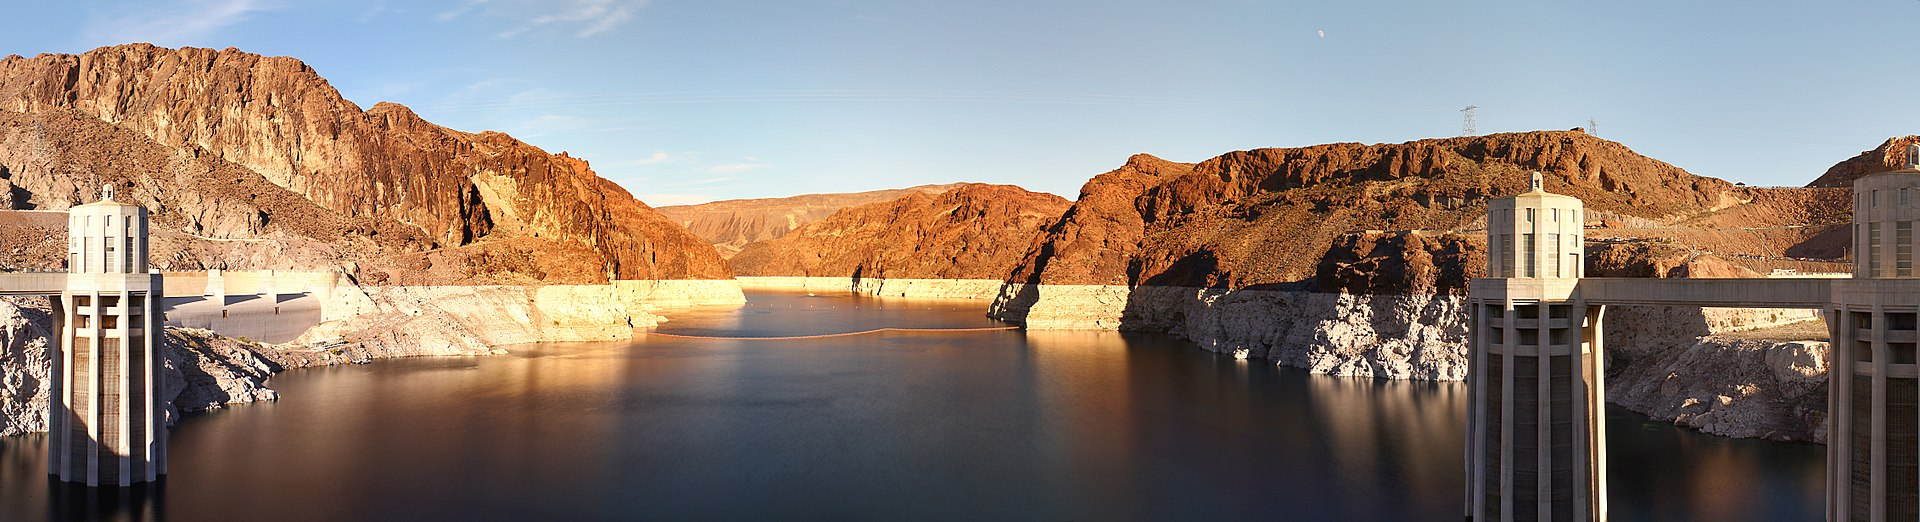
\includegraphics[width=13cm]{1.1 Lake Mead.jpg}

		\small \textit{Fig. 1.1 Lake Mead}
		\end{center}

	\subsection{Problem Restatement}
		Drought impact on water reservoirs is closely related to the environment conditions around the region, including rainfall.
		Lake Mead is mostly used to fulfill the need of people in Las Vegas, and thus the economic and geographic as well as the wastewater
		dealing facilities should also be taken into consideration.

		To analyze the impact and the solutions, the problem is divided into 4 parts:
		\begin{itemize}
			
			\item Finding out the factors affecting the elevation of Lake Mead and the relationship between them.
			\item Discussing the pattern of drought periods according to the data provided and predicting the water level in Lake Mead in year 2025,
			2030, and 2050 according to data from both the most recent drought period and that from 2005 to 2020, and finally selecting a 
			better one in these two ones.
			\item Making predictions on people's demand for water to decide the impact of wastewater recycling on future shortfalls and describing 
			our plan of wastewater recycling.
			\item Introducing the policies and recommadations from our plan based on the researches above.
		\end{itemize}

	\subsection{General Assumptions}
		\begin{itemize}
			\item \textbf{Climate differences in different parts of the lake is neglected.}
			
			Though the lake has an irregular shape, for the lake is only 112 miles in width, the climate differences can be ignored. \cite{Lake Mead}

			\item \textbf{The quantity of flow of the Colorado River is an average number.} \cite{Colorado River}

			\item \textbf{Glen Canyon Dam and other upstream dams don't affect Lake Mead.}
			
			Glen Canyon Dam, located in the upstream of the Colordo River is about 253 kilometers away from Lake Mead, so its impact can be ignored. \cite{List of Dams} \cite{Glen Canyon Dam}

			\item \textbf{Davis Dam doen't affect Lake Mead either. }
			
			Although the distance between Lake Mead and Davis Dam is less than 100 kilometers, it is located in the downstream, so the impact can
			also be ignored. \cite{List of Dams} \cite{Davis Dam}

			\item \textbf{The quantity of flow of the tributaries of the Colorado River is a constant number.}
			
			By seaching the official website and reading the documents, we learnt that the quantity of flow is relatively constant, so we assume that the number is stable in all seasons. \cite{Colorado River} \cite{Muddy River} \cite{Virgin River}

			\item \textbf{The quantity of flow is the same as the average data over the year.}
			
			To maintain stability of our model, we use the average data over the year for analyzing. 

			\item \textbf{The rainfall can be ignored.}
		\end{itemize}

\newpage
\section{Overall Analysis}

	\subsection{Problem Overview}
		
		At maximum capacity, Lake Mead is 112 miles long, 532 feet at its greatest depth, has a surface elevation of 1,221.4 
		feet above sea level and 247 square miles of surface area, and contains 26.12 million acre-feet of water.The lake has
		remained below full capacity since 1983 due to drought and increased water demand, so it is necessary to find a way
		which can maximize its water usage rate. \cite{Lake Mead}
		
		From the map given by Google, we drew the pictures and made the following conclusions:
		
		\begin{center}
		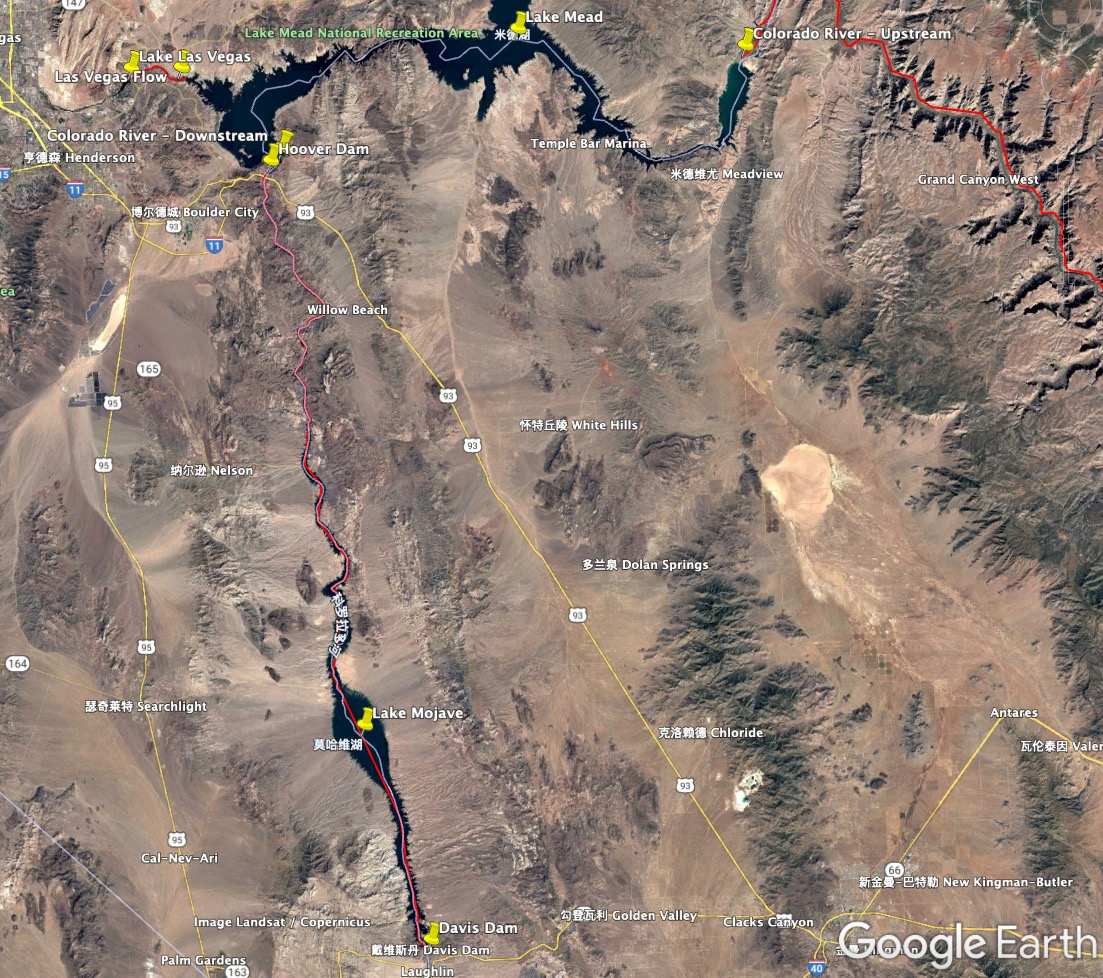
\includegraphics[height=4.2cm]{2.1a Lake Mead, Glen Canyon Dam and Davis Dam.jpg}
		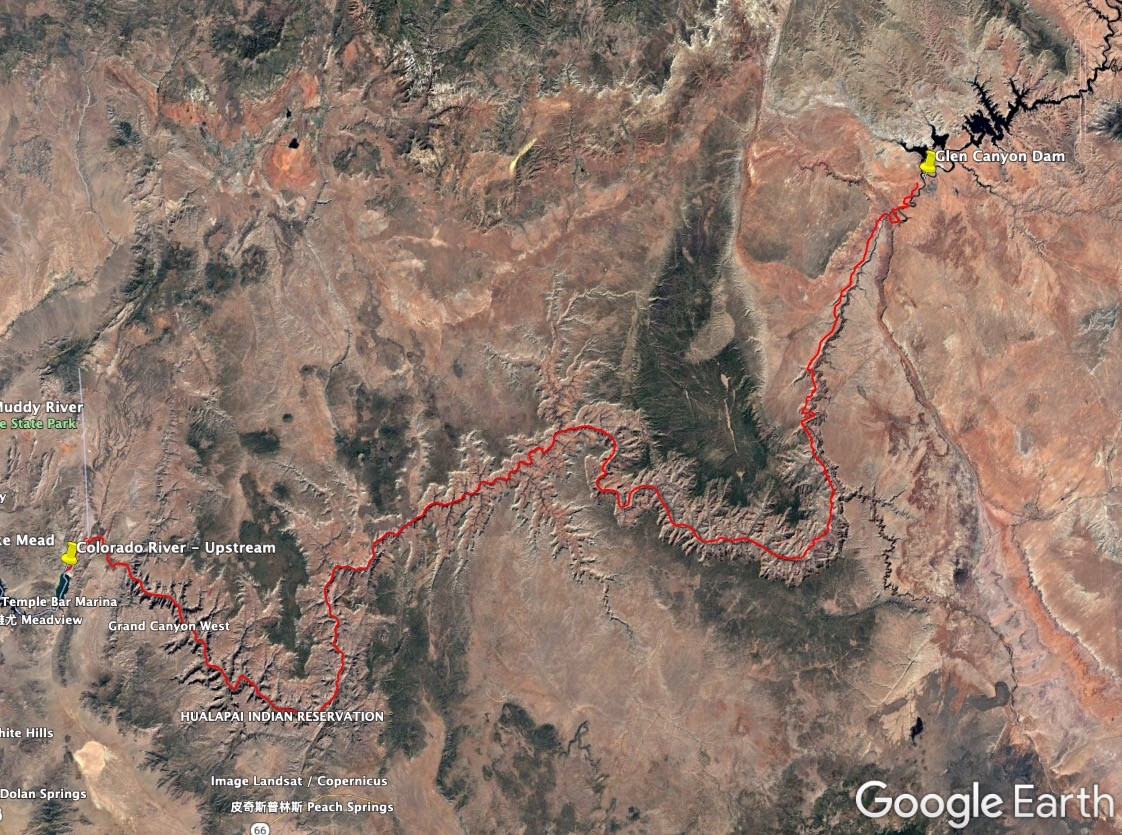
\includegraphics[height=4.2cm]{2.1b Lake Mead, Glen Canyon Dam and Davis Dam.jpg}
		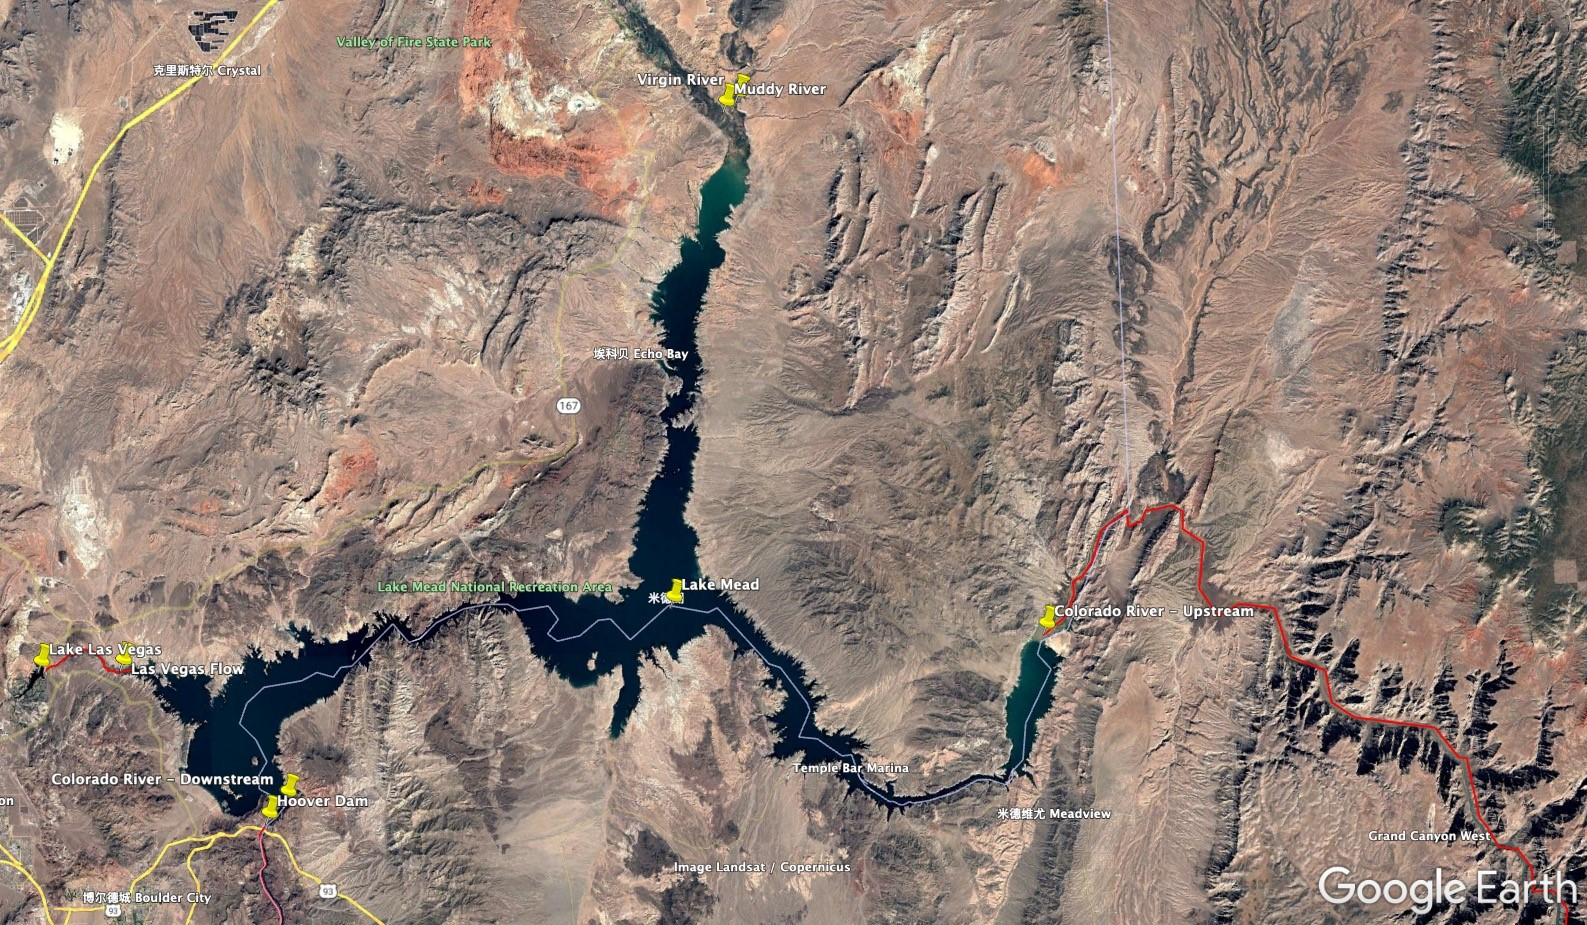
\includegraphics[width=10.5cm]{2.1c Lake Mead, Glen Canyon Dam and Davis Dam.jpg}

		\small \textit{Fig. 2.1 Lake Mead, Glen Canyon Dam and Davis Dam}
		\end{center}

		From these pictures, we found the basic flowing information of Lake Mead: the major source is from the Colorado River, so we can ignore the other tributaries. What's more, the Hoover Dam blocked most of the stream, so we only need to take Hoover Dam into consideration.
		
		\begin{center}
			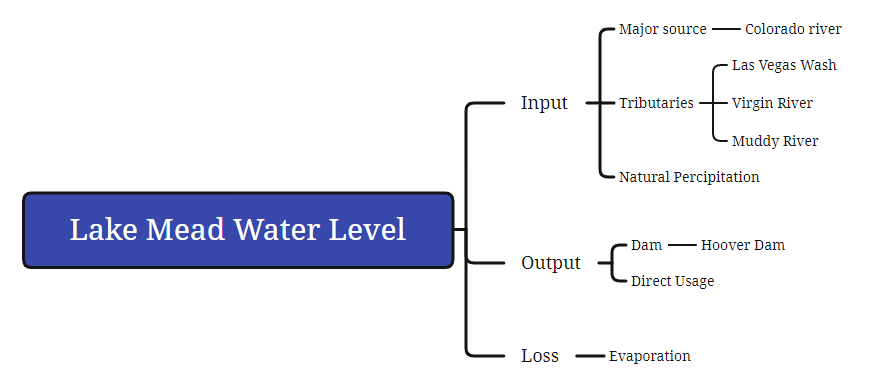
\includegraphics[width=12cm]{2.2 Inflow, outflow and loss of Lake Mead.png}
			
			\small \textit{Fig. 2.2 Inflow, outflow and loss of Lake Mead}
		\end{center}
		
		
		According to these facts, there are some necessary things to do:
		
		\begin{itemize}
			\item discover the factors which influence inflow, outflow and loss.
			
			\item discover the imapct of each factor on the river's volume.
		\end{itemize}
			
	\subsection{Notation}
			\begin{tabular}{lll}
				\hline
				Symbol&Stands For&Unit\\
				\hline
				$I$&Inflow&$\rm{m^3/s}$\\
				$O$&Outflow&$\rm{m^3/s}$\\
				$EV_{lake}$&Evaporate&$\rm{m^3/s}$\\
				$T$&Temperature&$\rm{K}$\\
				$t$&Time&/\\
				$Q_{\rm{Wash}}$&Quantity of Flow of Las Vegas Wash&$\rm{m^3/s}$\\
				$Q_{\rm{Virgin}}$&Quantity of Flow of Virgin River&$\rm{m^3/s}$\\
				$Q_{\rm{Muddy}}$&Quantity of Flow of Muddy River&$\rm{m^3/s}$\\
				$H\in \left[0, H_{\max}\right]$&Water Level&$\rm{m}$\\
				$Q_{\rm{Dam}}\in\left[0,Q_M\right]$&The Amount of Water Released from the Dam&$\rm{m^3/s}$\\
				$Q_{\rm{Rain}}$&Rainfall Quantity&$\rm{m^3/s}$\\
				\hline
			\end{tabular}	
		
	\subsection{Result}
		The quantity of flow is closely to the vaporization of water. We found a formula decribing the evaporation of water and its relationship with temperature and air pressure: \cite{Vapor Pressure}
		
		\begin{align*}
			\lg\frac{p_2}{p_1}&=-\frac{\Delta H_\text{vap}}{2.303R} \left(\frac{1}{T_2}-\frac{1}{T_1}\right)\\
			p&=10^{\left(-\frac{\Delta H_{vap}}{2.303R}\times\frac{1}{T}+\text{Const}\right)}\\
			n&=\frac{pV}{RT}=\frac{\rho ghV}{Rt}=\frac{A}{T} e^{\left(-\frac{B}{T}\right)}\\
			n\%&=p+C=10^{\left(-\frac{\Delta H_{\text{vap}}}{2.303R}\times\frac{1}{T}+\text{Const}\right)}+C\\
		\end{align*}
	
		\begin{center}
			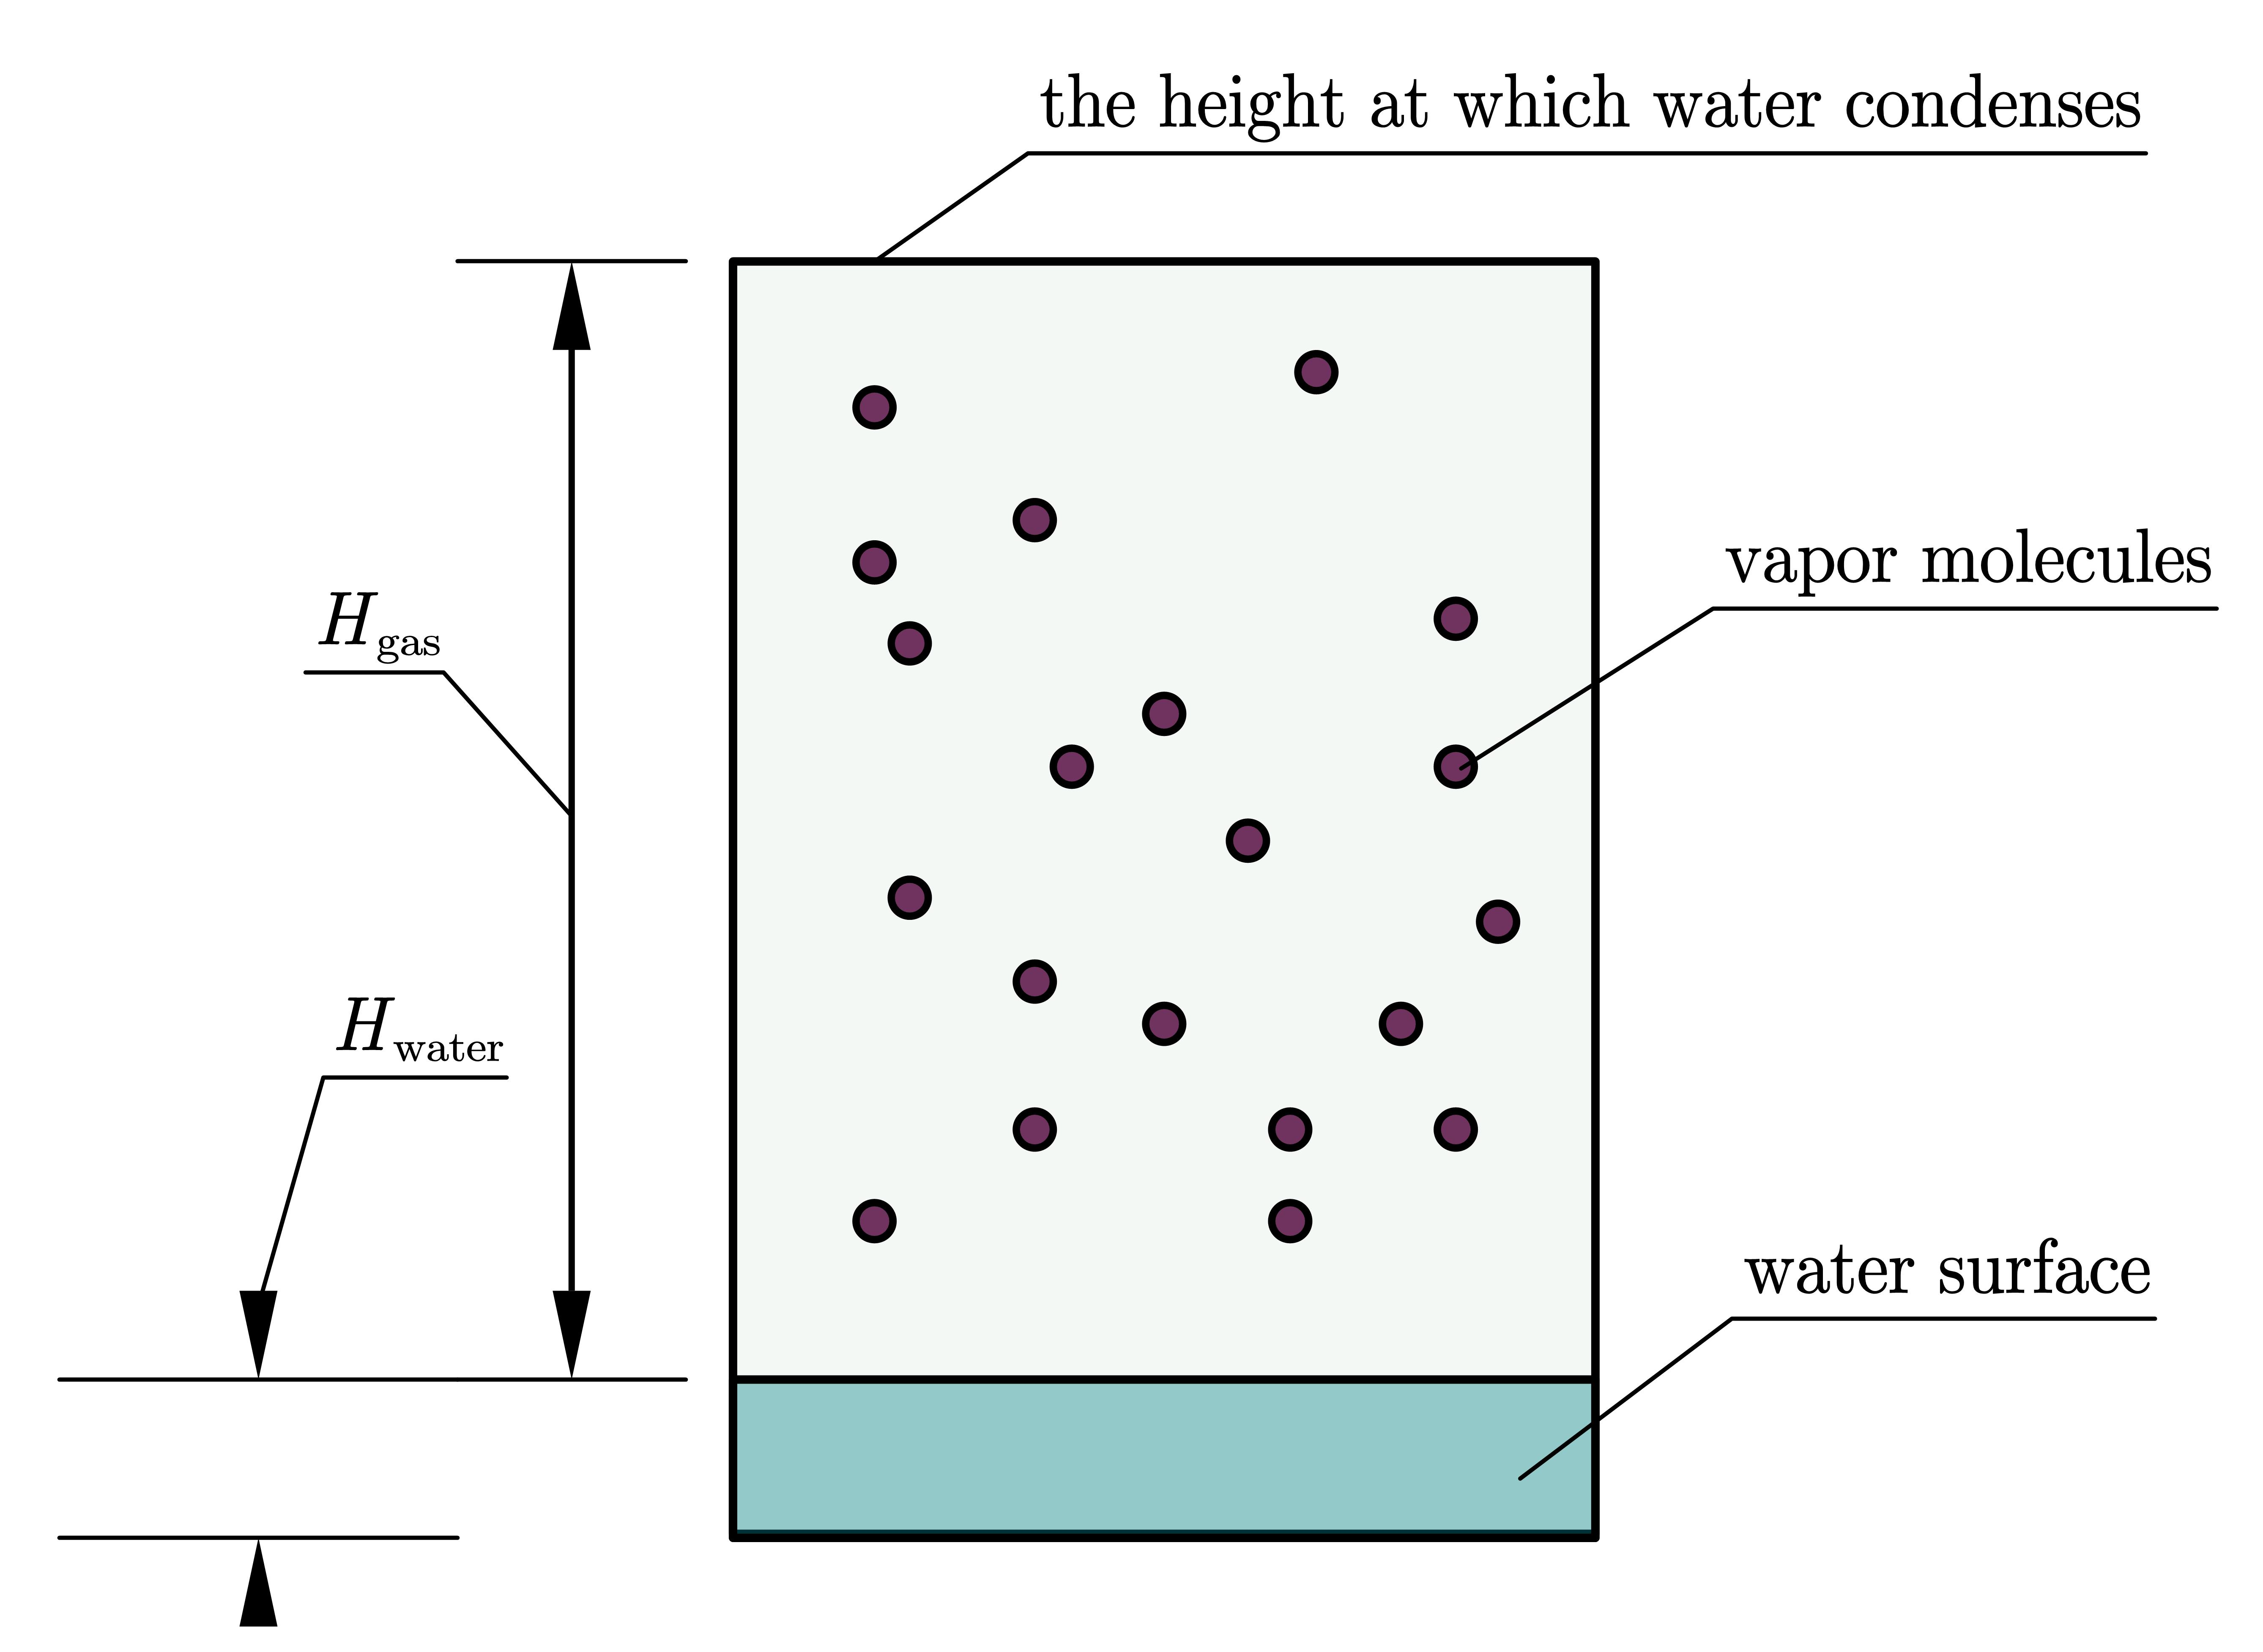
\includegraphics[height=4cm]{2.3 Describing Vaporization.jpg}
			
			\small{\textit{Fig. 2.3 Describing Vaporization}}
		\end{center}
		
		According to this formula, we discovered three formulas.
		
		$$\begin{array}{rcl}
			\dfrac{\mathrm{d}EV}{\mathrm{d}t}&\propto&S_{\text{Lake}}\\\\
			\dfrac{\mathrm{d}EV}{\mathrm{d}t}&\propto&\dfrac{1}{x}\cdot\exp\left(\dfrac{1}{x} \right)\\
			S_{Lake}&\leftarrow& V_{\text{Lake}}\\	
		\end{array}$$
		
		Secondly, by investigating the quantity of flow and the relationships between Lake Mead and its inflow,we listed out four formulas.
		
		$$\begin{array}{rcl}
			V_{Lake}&=&I-O-EV(V_{\text{Lake}})\\
			I&=&Q_{\text{Wash}}+Q_{\text{Virgin}}+Q_{\text{Muddy}}+Q_{\text{Rain}}\\
			O&=&Q_{\text{Dam}}\\
			H&=&H_{\text{Lake}}\\
		\end{array}$$
		\subsection{Depth-Area}

	The area of Lake Mead is 640, 000, 000$\rm{m}^2$ and its depth is 162$\text{m}$ \cite{Lake Mead}, so the length of the top equals the square root of the area. ($l_{\text{top}}=\sqrt{6.4\times{10^8}} \rm{m}\approx25298.2\rm{m}$)

	Assume that the shape of the lake can be simplified into a model like the images below:
	
	\begin{center}
		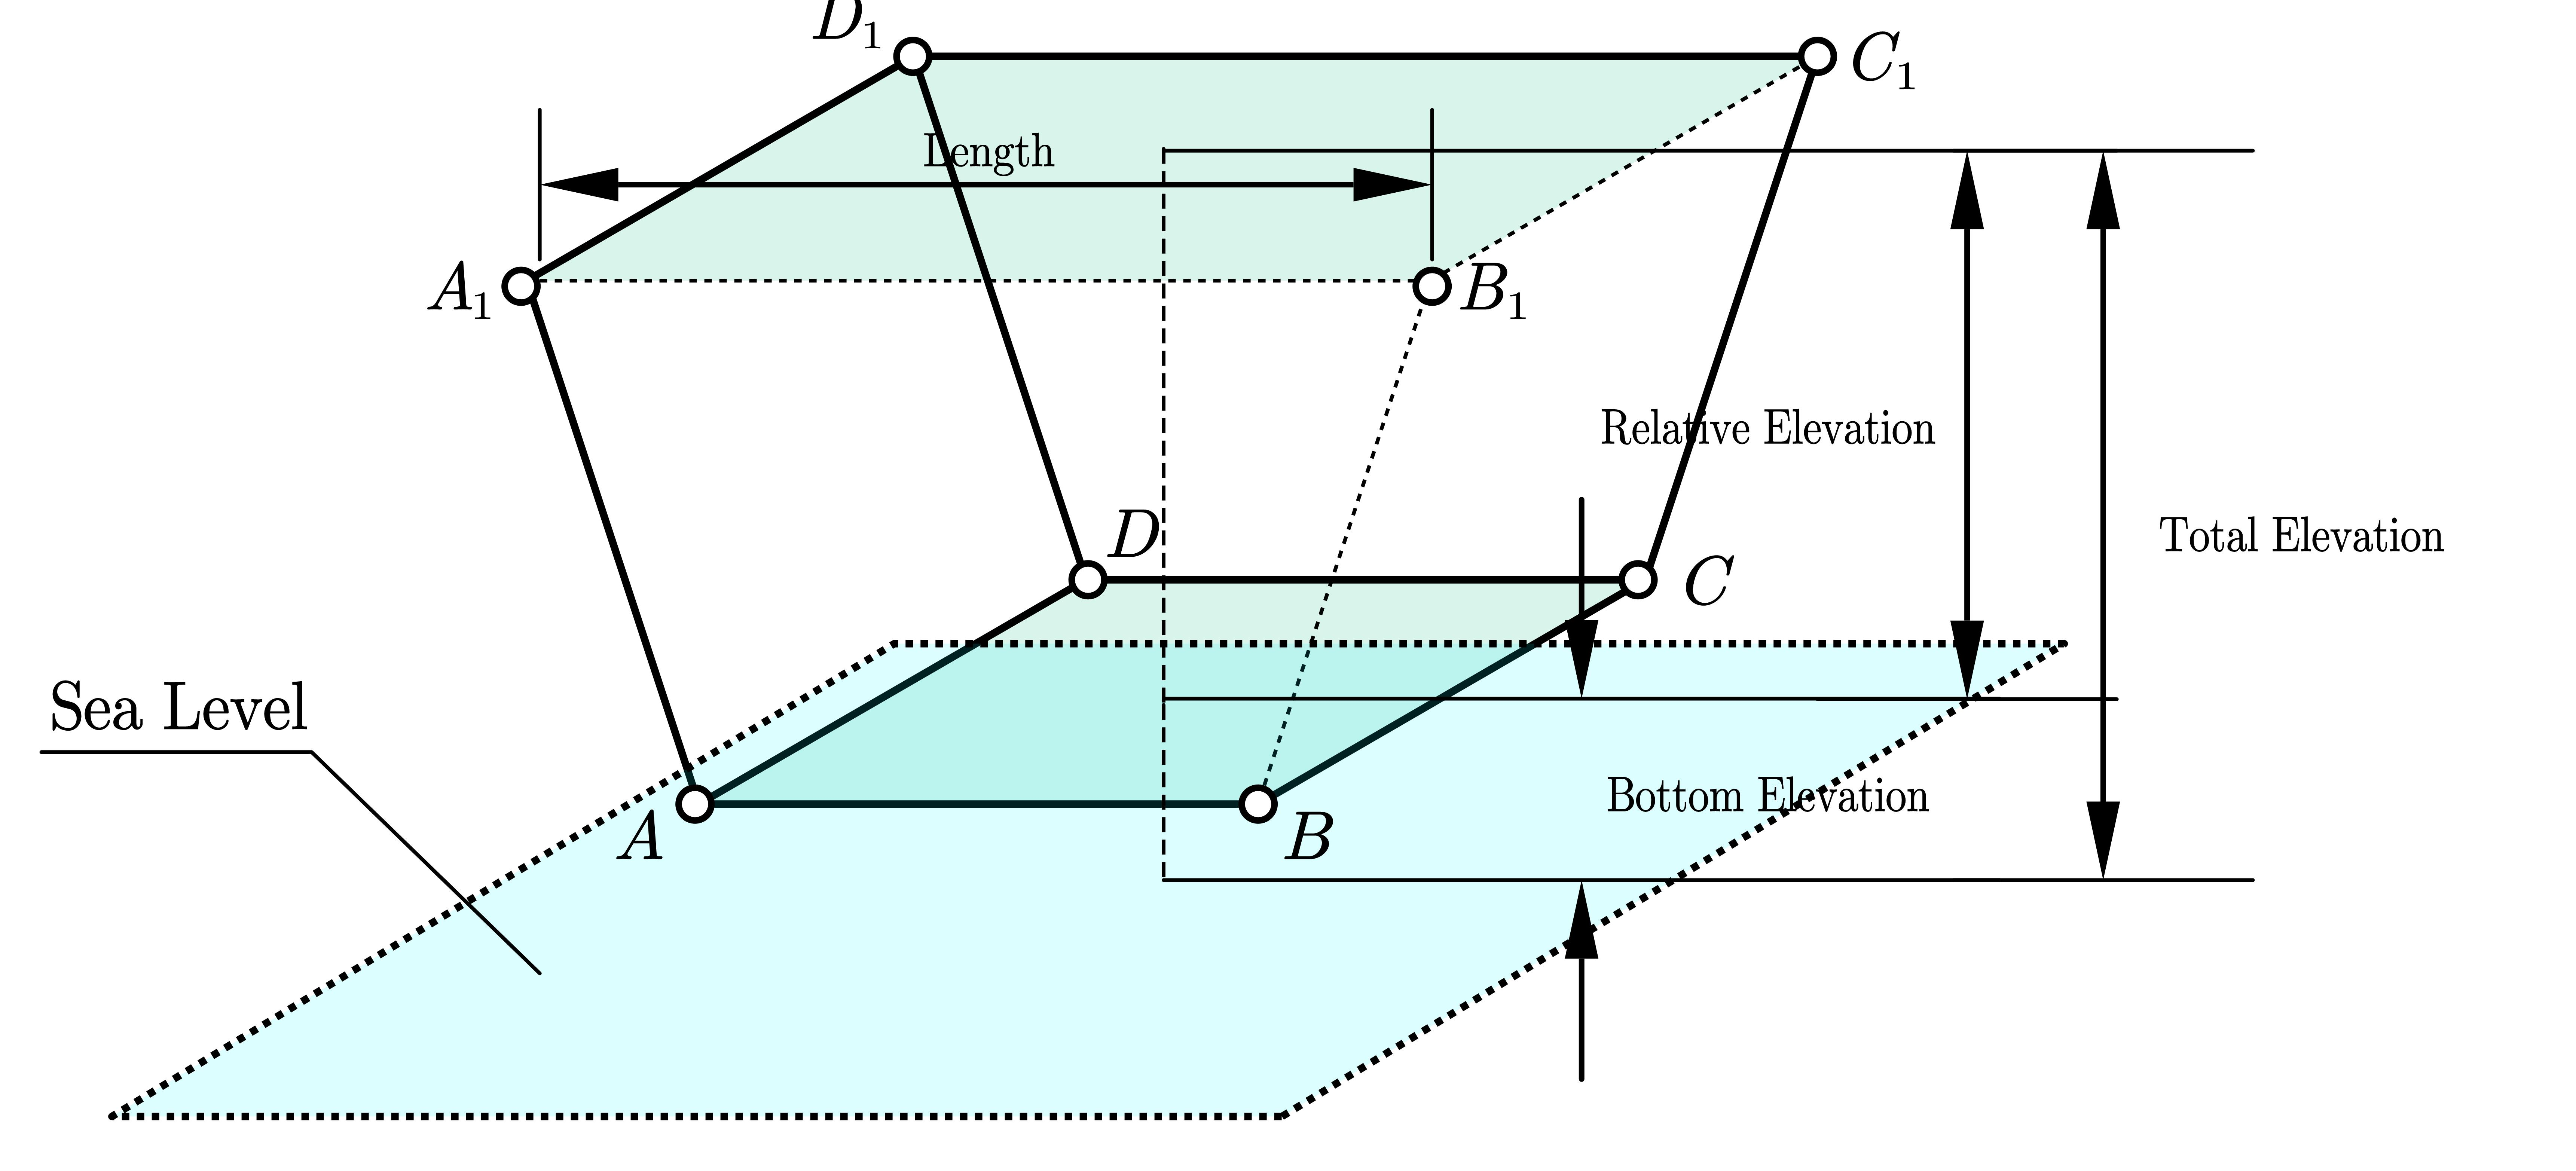
\includegraphics[width=10cm]{2.4 Model labeled with Elevation.jpg}
		
		\small\textit{Fig. 2.4 Model labeled with Elevation}
		
		
		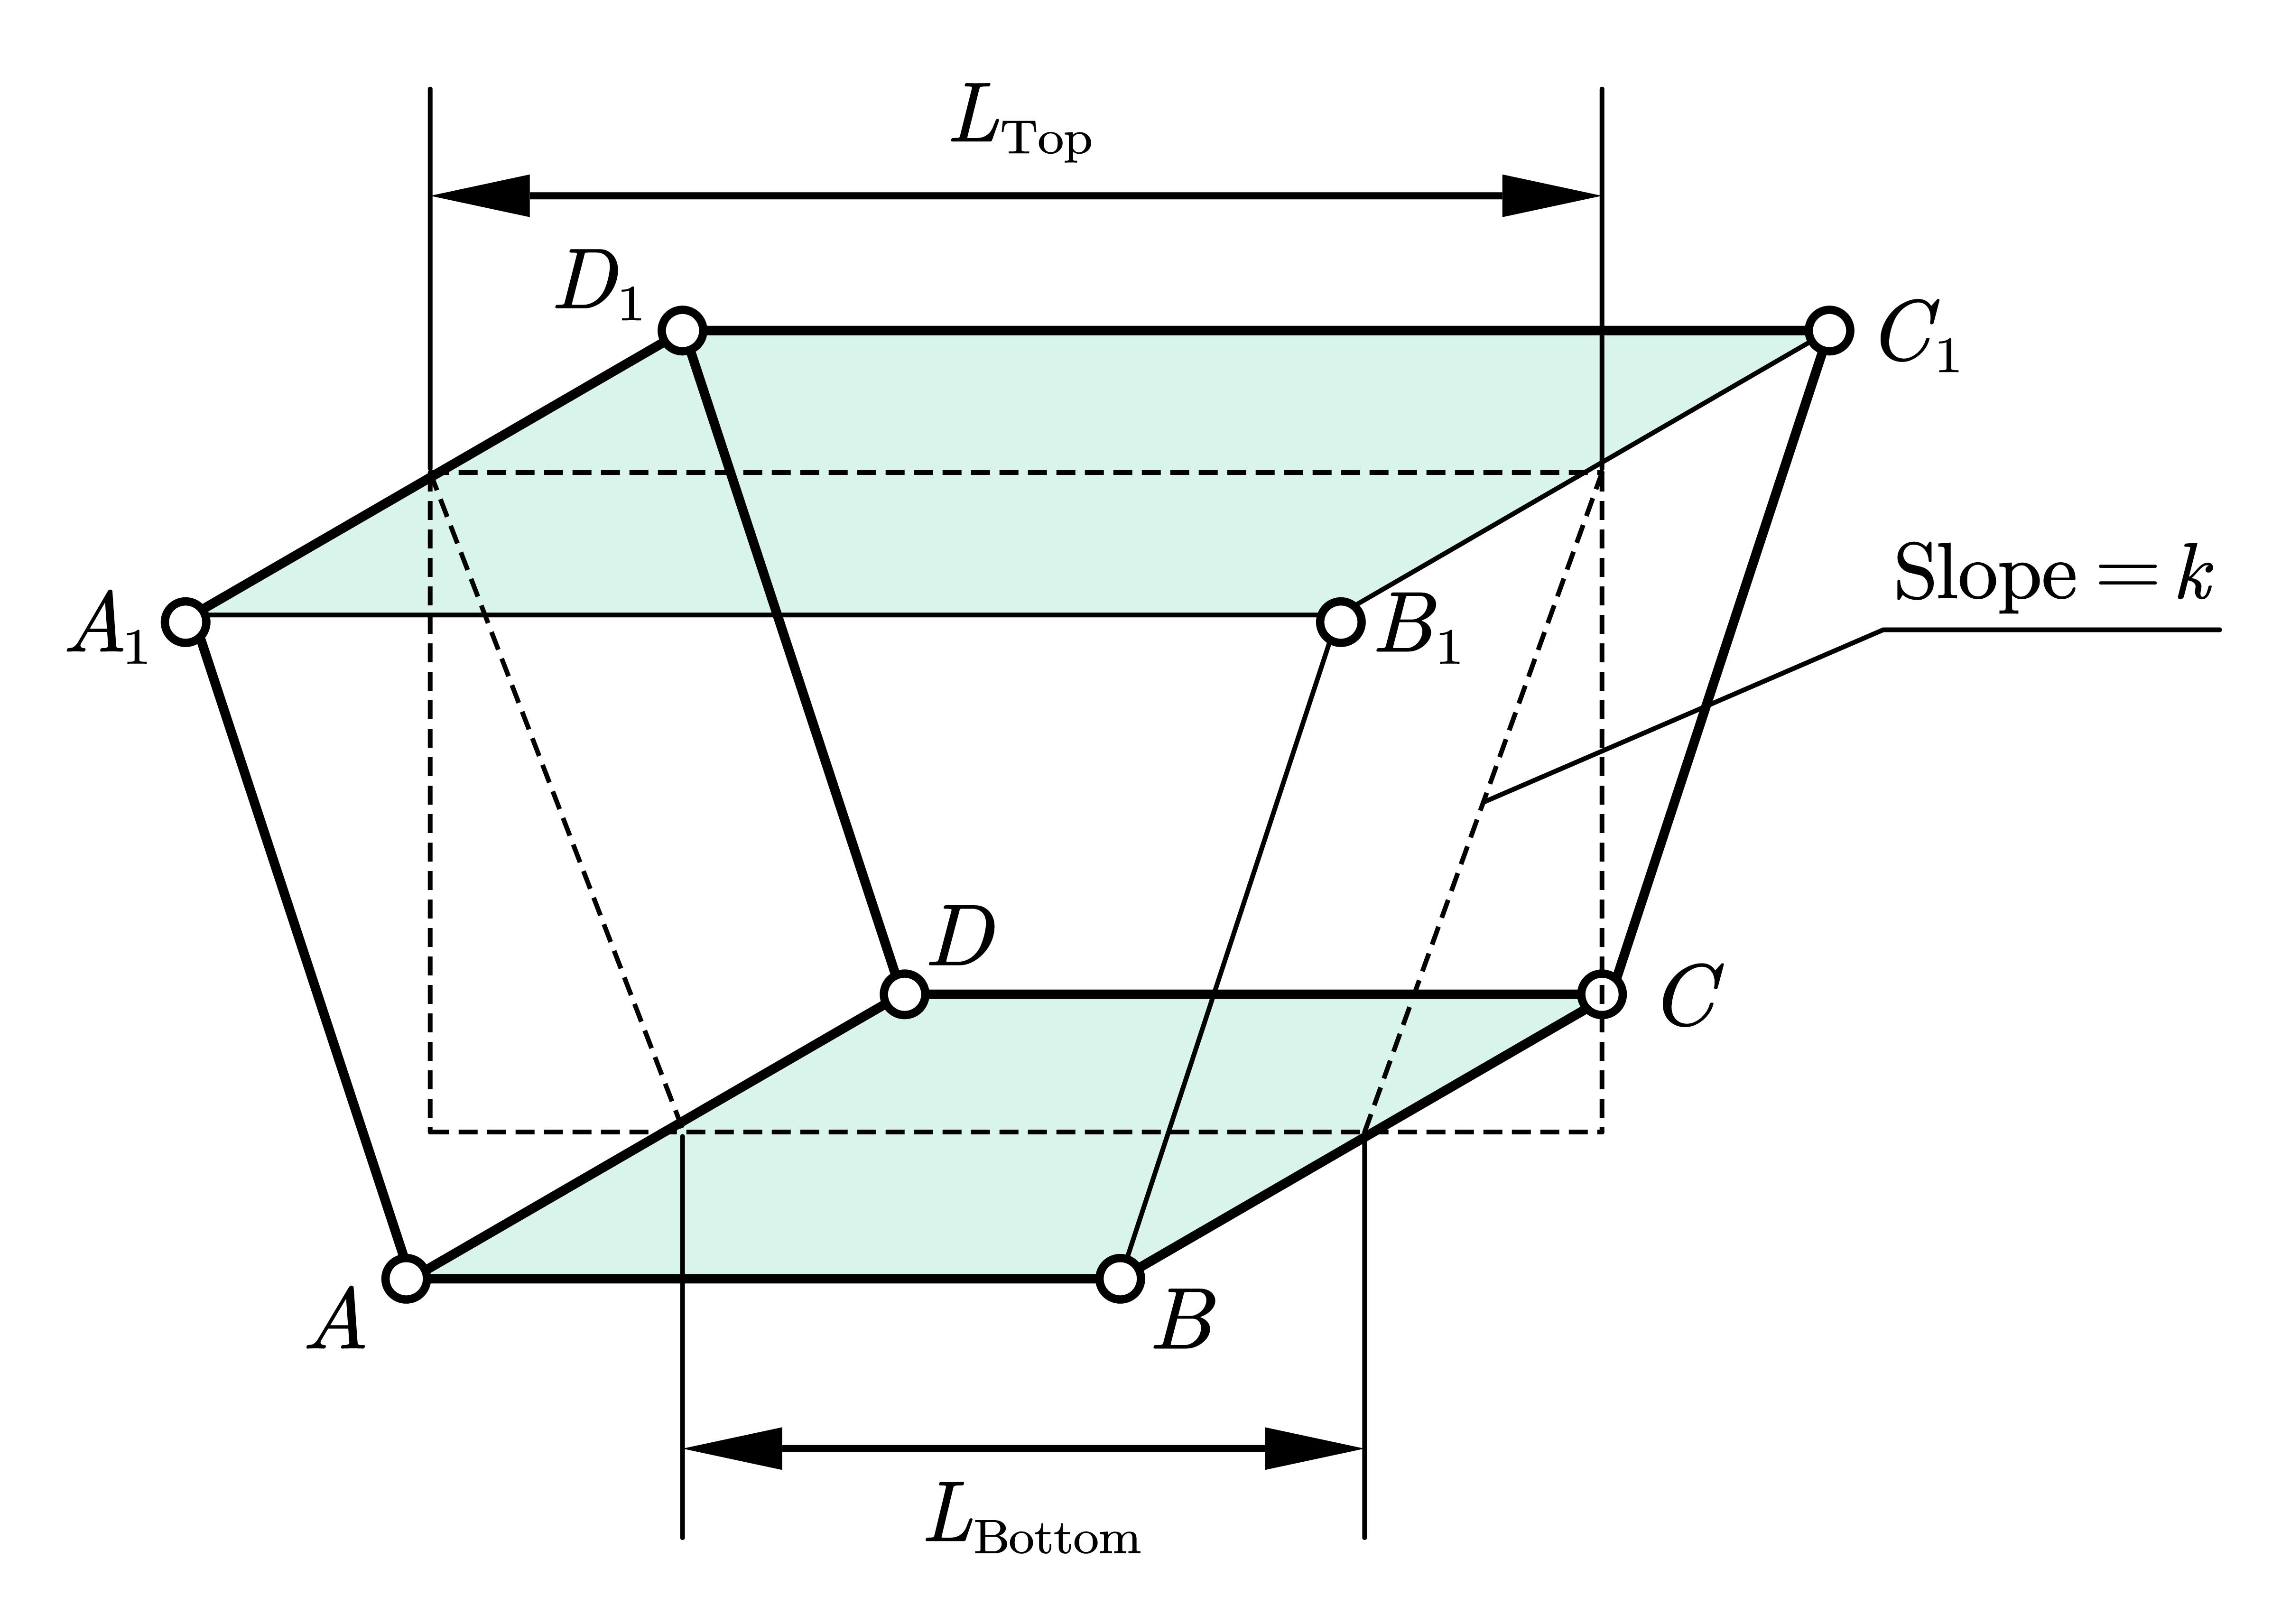
\includegraphics[width=10cm]{2.5 Model labeled with Length and Slope.jpg}
		
		\small\textit{Fig. 2.5 Model labeled with Length and Slope}
	\end{center}

	We drew a plot between h and the square root of area ($l$), and found a linear function. The slope of this function $k_0$  is 1.473.
	
	Assume that the slope of the edges $AA_1$, $BB_1$, $CC_1$ and $DD_1$ is $k$, and we can find that:
	
	\begin{align*}
		k&=2\frac{\Delta h}{\Delta l}=2k_0=2.946\\
		k&=\frac{324}{l_\text{top}-l_\text{bottom}}\\
		l_{\text{bottom}}&=25188.2\rm{m}.\\
		area&=\left(25188.2+\frac{h}{1.473}\right)^2. \cite{Water Level Data}\\
	\end{align*}
	
	($h$ refers to the distance between a certain depth and the bottom of the lake)

	\subsection{Verification}

	In the analysis of the first part, we discuss the loss of water due to evaporation based on the formula of Water Vapor Equilibrium. Now we need to do more to discuss the accuracy of this formula.
	
	We used the data from Bureau of Reclamtion \cite{Storage Data} and recorded the evaporation condition of Lake Mead. After analyzing the relationship, we drew a chart to find its degree of difference between the formula and the data's pattern.
	
	\begin{center}
		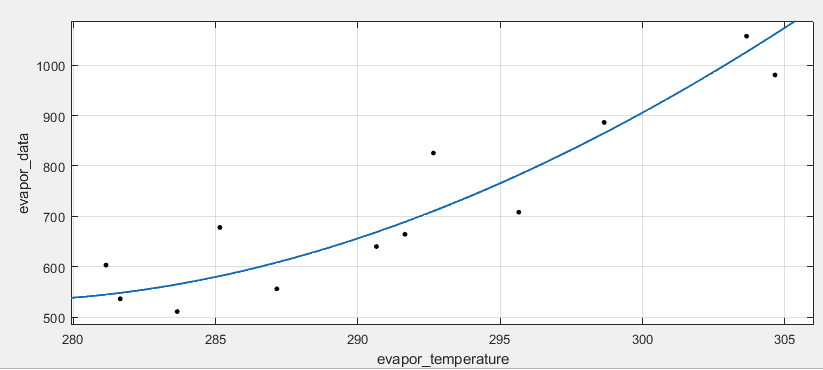
\includegraphics[width=10cm]{2.6 Pattern provided by data.png}
		
		\small \textit{Fig. 2.6 Pattern Provided by data}
	\end{center}

	From this chart, we deduce that the mathematical formula in the former part fits well with the official data: the R-square is only at a level of 0.8664 and the RMSE is 72.08.

	\begin{center}
		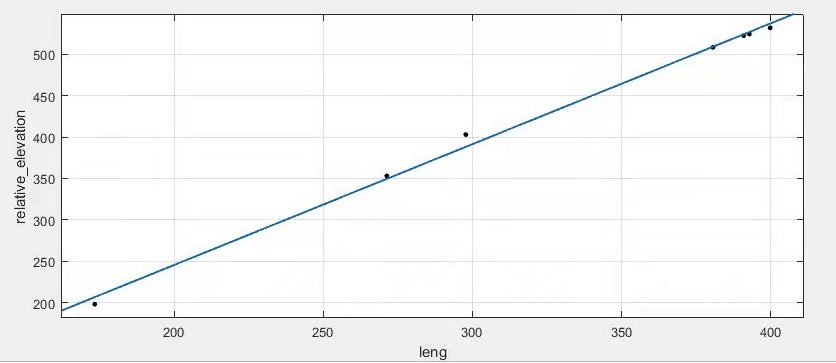
\includegraphics[width=10cm]{2.7 The Relationship between Relative Elevation and Length.jpg}

		\small \textit{Fig. 2.7 The Relationship between Relative Elevation and Length}
	\end{center}

	We obtained data from the official website of Lake Mead \cite{Storage Data}, thus plotting it using MATLab Curve Fitting. From Fig. 2.7, we can see that the relative elevation of Lake Mead has a rather linear relationship with the length, i.e. the square root of the area. Therefore, we can infer the correctness of the prismatic shape as assumed above.

\newpage
\section{Dealing with Drought}

	\subsection{Data Analysis}
		After analyzing the data given, we drew some figures to show the pattern of Lake Mead.
		
		\begin{center}
		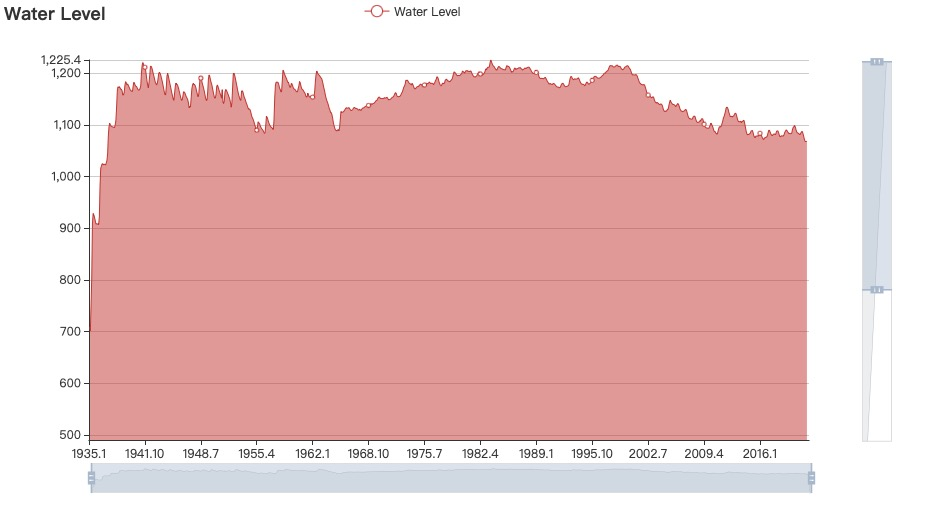
\includegraphics[width=10cm]{3.1 Water Level in Inches.jpg}

		\small \textit{Fig. 3.1 Water Level in Inches}
		\end{center}
		
		Plotting all the data provided into a single line plot creates Fig. 3.1. The minimum during a small period (a year) is significant and will be discussed later. During the first few years of Lake Mead (1935-1939), the water level took a steep rise from approx. 700 ft to approx. 1100 ft. Years 1955-1957 saw the first drought of Lake Mead, reaching a minimum of 1083.57 ft in March, 1956. Lake Mead then experienced a short period of normal water level until the drought from 1964-1966. A water level of 1088 ft was reached in 1964.12 and 1965.3. Rising steadily since, the water level peacked in 1983.7 with 1225.4 ft. The water level was steady until the 21st century, and the Water Level drops steadily. In other words, Lake Mead was in a drought since then.
		
		\begin{center}
		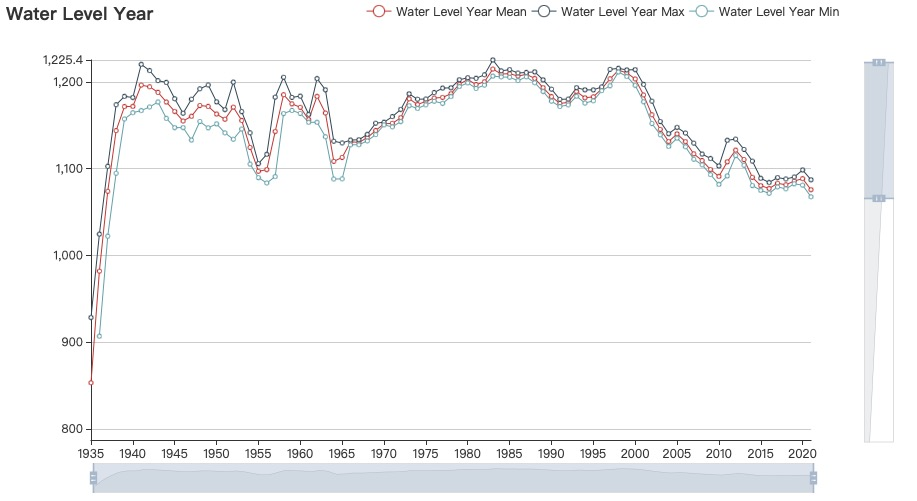
\includegraphics[width=10cm]{3.2 Mean, Max. and Min. of Water Level in Inches by Year.jpg}

		\small \textit{Fig. 3.2 Mean, Max. and Min. of Water Level in Inches by Year}
		\end{center}
		
		Then, taking the maximum and minimum water level into consideration (Fig 3.2), the range (the difference
		between maximum and minimum) usually increases when the water level rises or falls significantly, and 
		decreases when the water level is steady.
		
		\begin{center}
		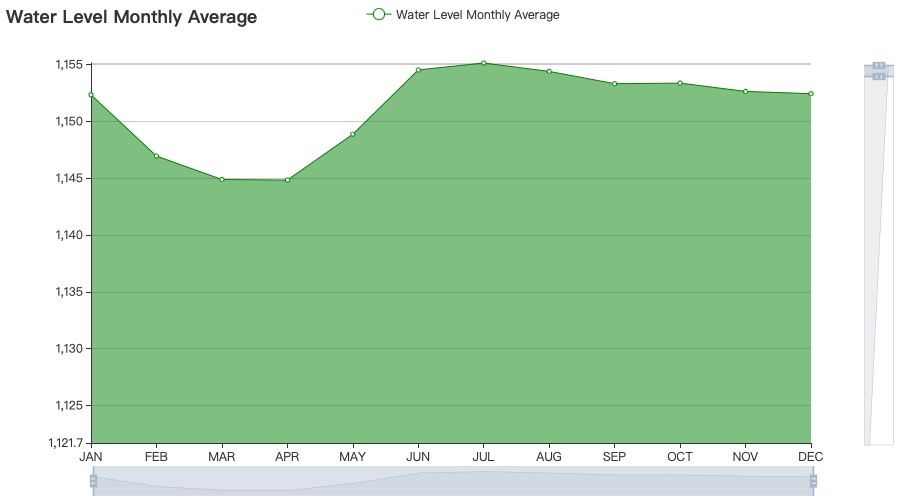
\includegraphics[width=10cm]{3.3 Mean of Water Level in Inches by Month.jpg}

		\small \textit{Fig. 3.3 Mean of Water Level in Inches by Month}
		\end{center}
		
		According to Fig. 3.3, it is obvious that the water level drops significantly in the gap between Winter and
		Spring, reaching a minimum of 1,145 ft avg. in March and April. After the drop, the water level rises an 
		peaks in July with an average of 1,155 ft. It decreases steadily in Autumn and Winter, and the pattern
		continues almost every year. However, the pattern became inconspicuous before, during and after a drought.
		
	\subsection{Definition of Drought}
		We used three different ways to define drought index:
		\begin{itemize}
			\item We identify the drought index($D_1$) as $H_\text{last month}-H_\text{this month}$, so $D_n$ is the arithmetic mean 
			value of the months.
			\item We identify the drought index($D_2$) as $\dfrac{H_\text{this month}}{H_\text{last month}}$, so $D_n$ is the  geometric
			mean value of the months.
			\item We identify the drought index($D_3$) as the range ($n$) of the average water level in the years which the year when water
			level is the highest is earlier than the year when water level is the lowest.
			
			If there are years that fulfill three statements at the same time, we identify the time period as drought.
		\end{itemize}

		From these three statements, we ge the following pattern.
		
		\begin{center}
		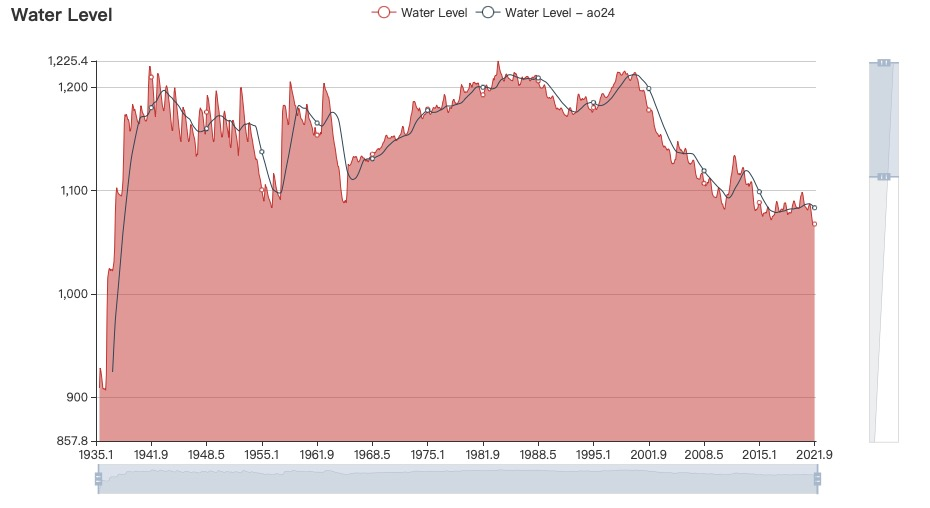
\includegraphics[width=10cm]{3.4 Water Level and Water Level (ao24) in Inches.jpg}

		\textit{Fig. 3.4 Water Level and Water Level (ao24) in Inches}
		\end{center}
		
		As shown in Fig. 3.4, a data of the average water level of the past 24 months is caculated and plotted on the same plot 
		as the water level. It is observed that the small peaks and valleys are smoothed while the big ones are postponed. Therefore,
		we decided to define the drought (in another way) using the ao24 and relative drop, or:
		$$
		a_x\leq AO24_x \cdot (1+0.5\%).
		$$
		The $0.5\%$ is determined by the relative drop of commonly accepted droughts.


	\subsection{Differences between Droughts}
		\begin{itemize}
			\item The recent drought has a lower rate of elevation decrease, but lasts longer. Therefore, it has a higher total elevation
			decrease.
			\item The monthly elevation is going up and down in the recent drought (though the extent of decrease is much higher 
			than that of increase), while past droughts almost decreasing almost all the time. 
		\end{itemize}

	\subsection{Assumption}
		\begin{itemize}
			\item Percipitation will not be taken into account, as the rain is too little to have impact on the water level (see Fig. 3.5). What's more, the desert climate leads directly to great evaporation of lake water, which is significantly bigger than the percipitation.
			\item  The change of temperature over years will not be taken into consideration either, for the change over years is too small. The average temperature of a day will be calculated as the mean of maximum and minimum (see Fig. 3.5).
			\item The use of water, which is a part of human factor, will be a constant. However, the constant can change over time as policies and regulations tighten or losen. As shown in Fig. 3.6, the "sudden"  increase of water level can be interpreted by a change of water using policy, and can be shown in the model by a change of the constant.
		\end{itemize}

		\begin{center}
			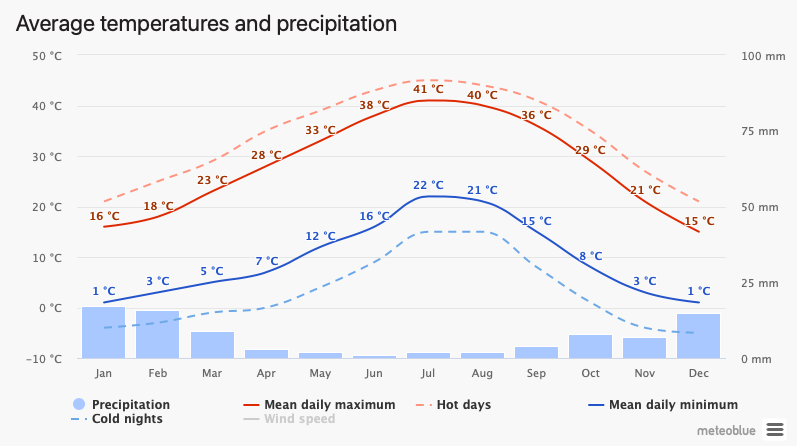
\includegraphics[width=10cm]{3.5 Average Temperatures and Percipitation of Lake Mead.png}
			
			\small \textit{Fig. 3.5 Average Temperatures and Percipitation of Lake Mead \cite{Temperature and Percipitation Data}}
			
			~\\

			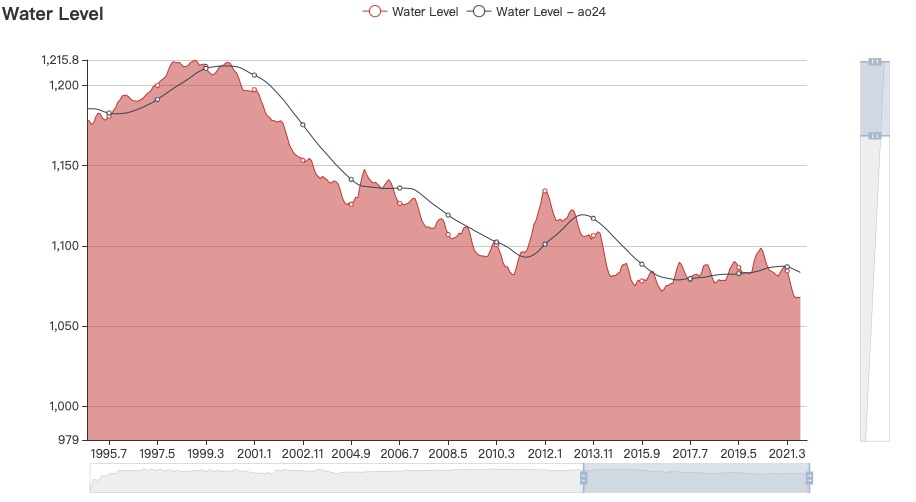
\includegraphics[width=10cm]{3.6 Sudden Increase of Water Level in 2010-2012.jpg}
			
			\small \textit{Fig. 3.6 Sudden Increase of Water Level in 2010-2012}
		\end{center}
		
	\subsection{Cycle-Linear Model}

		In this model, our target is simulating a cycle process of linear functionsso as to predict the elevation level in 2025, 2030 and 2050.

		From Sep to Dec of 2021, the data does not follow the rule due to various reasons. Thus, this period will not be studied. Excluding previously mentioned data, according to historical elevation level data of Lake Mead, a periodic function can be got. 
			
		The first 3 month increase with slope of 4.55834 and constant is $1071.80001$. Therefore, the function is $H = 4.55834(T-1044)+1071.80001, T \in [1044, 1047)$.

		After that, there is a continuous 60 month decrease with a slope of -1.18813 and a constant of 1085.47503. The function is $H = -1.18813(T-1047)+1085.47503, T \in [1047, 1106)$.

		The overall cycle function is as following:

		$$H =
		\left\{
		\begin{array}{rclr}
		1.36667(T-1044)+1071.80001& \text{for} &T\in[1041,1044) & \text{Special (2021.09-11)}\\
		4.55834(T-1044)+1071.80001& \text{for} &T\in[1044,1047) & \text{Fast Increase}\\
		-1.18813(T-1047)+1085.47503& \text{for} &T\in[1047,1106) & \text{Decrease}\\
		F(T-63)-57.61278& \text{for} &T\in[1106, +\infty) & \text{Cycles}\\
		\end{array}
		\right.$$

		\begin{center}
			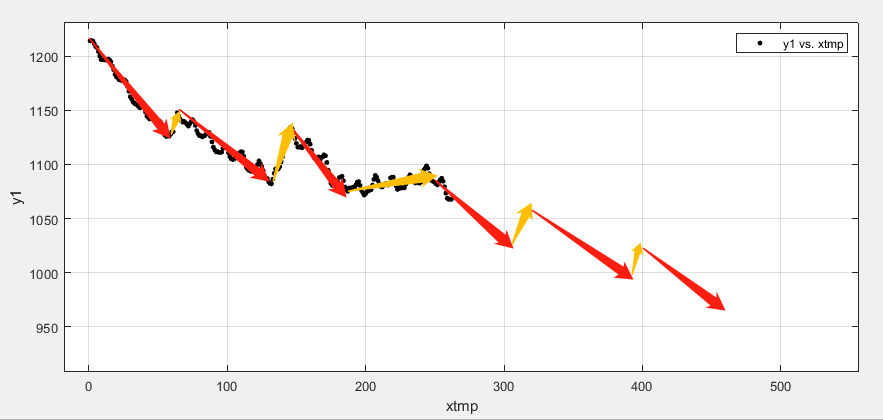
\includegraphics[width=10cm]{3.7 Cycles.png}
			
			\small \textit{Fig. 3.7 Cycles}
		\end{center}

		Thus, the results for 2025, 2030 and 2050 would be:

		~\\
		\begin{center}
		\begin{tabular}{ccccc}
			\hline
			Year&Water Level (Inches)\\
			\hline
			2025&1037.35577\\
			2030&984.49551\\
			2050&768.30195\\
			\hline
		\end{tabular}
		\end{center}
		~\\

	\subsection{Dynamic Model}

		In Model 2, our target is simulating a dynamic process so as to predict the future water levels. In this case, we do it based on recursion. As analyzed in the first part, the relationships of volume of the lake and other factors of the process can be determined mathematically, the accuracy and correctness of which has already been proven. As given in the assumptions, the temperature and other nature-based variables can be considered as constants in a single month. Therefore, our work is solving the differential equation and use historical data to determine the constants $D_1$ and $D_2$ as shown below:

		$$
		V=\exp (-C_2  t + D_1) + C_1 t + D_2.
		$$

		\begin{center}
		\includegraphics[width=10cm]{3.8 Fit of Function to Data.jpg}

		\small \textit{Fig. 3.8 Fit of Function to Data}
		\end{center}

		Here, we consider $C_1$ as the inflow of the Lake Mead. $C_1$ is calculated as $\dfrac{100}{96}$ of the Colorado river inflow, mius the human use of water, only considering Las Vegs, or $6.49191$ \cite{Water Use in Las Vegas}, minus the outflow of Hoover Dam \cite{Water Level Data}. $C_2$ is a function of temperature (to describe evaporation) as following:

		$$C_2 = A_1 \frac{\exp(-B / T)}{T} + A_2,$$

		where $A_1 = -9.187\mathrm{e}+07, A_2 = 1.225\mathrm{e}+05, B = 277.1$, as fitted using evaporation data previously.

		It's obvious that the constant $D_1$ directly determines the horizontal translation, while the vertical one is determined by $D_2$. And by using the convex property of the function, we can easily deduce that the function itself can be decided if two fixed points on the graph are given. In each step, we build an $X-Y$ coordinate in which the previous point is on the y-axis. Thus we get the following graph which displays the variation of constant $D_1$. 

		\begin{center}
		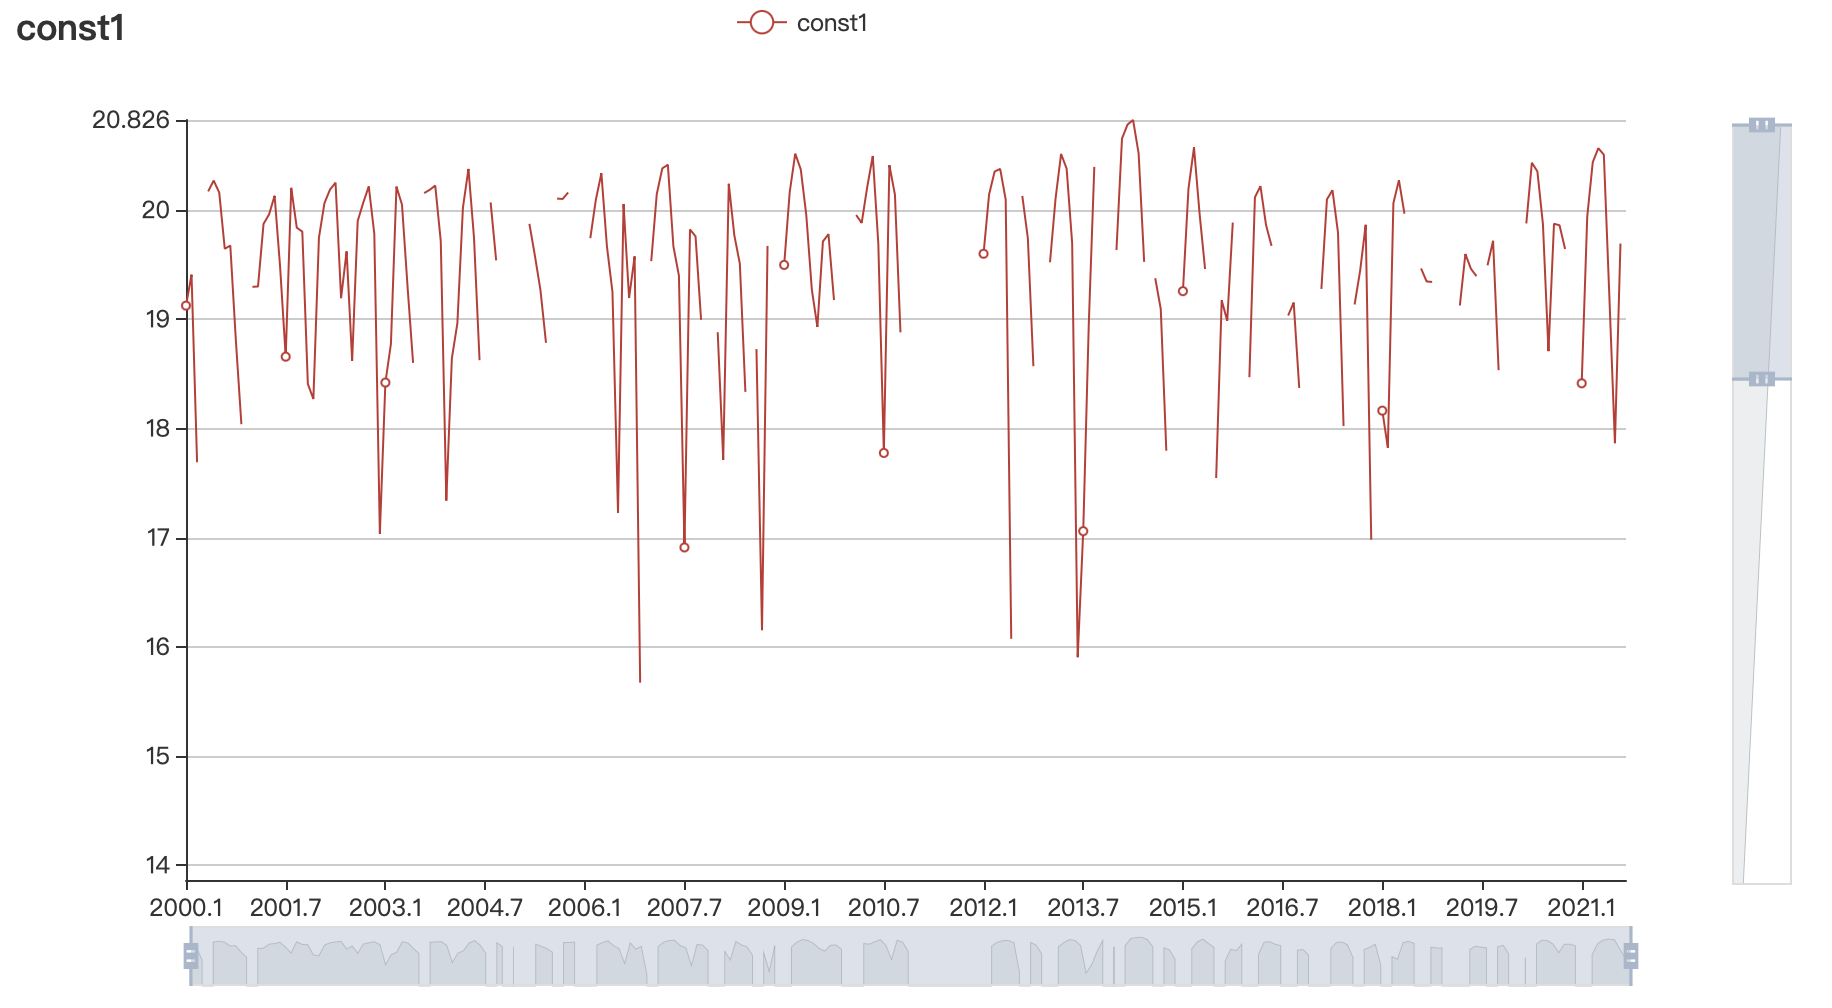
\includegraphics[width=10cm]{3.9 D_1 over time.jpg}

		\small \textit{Fig. 3.9 $D_1$ over time}

		~\\

		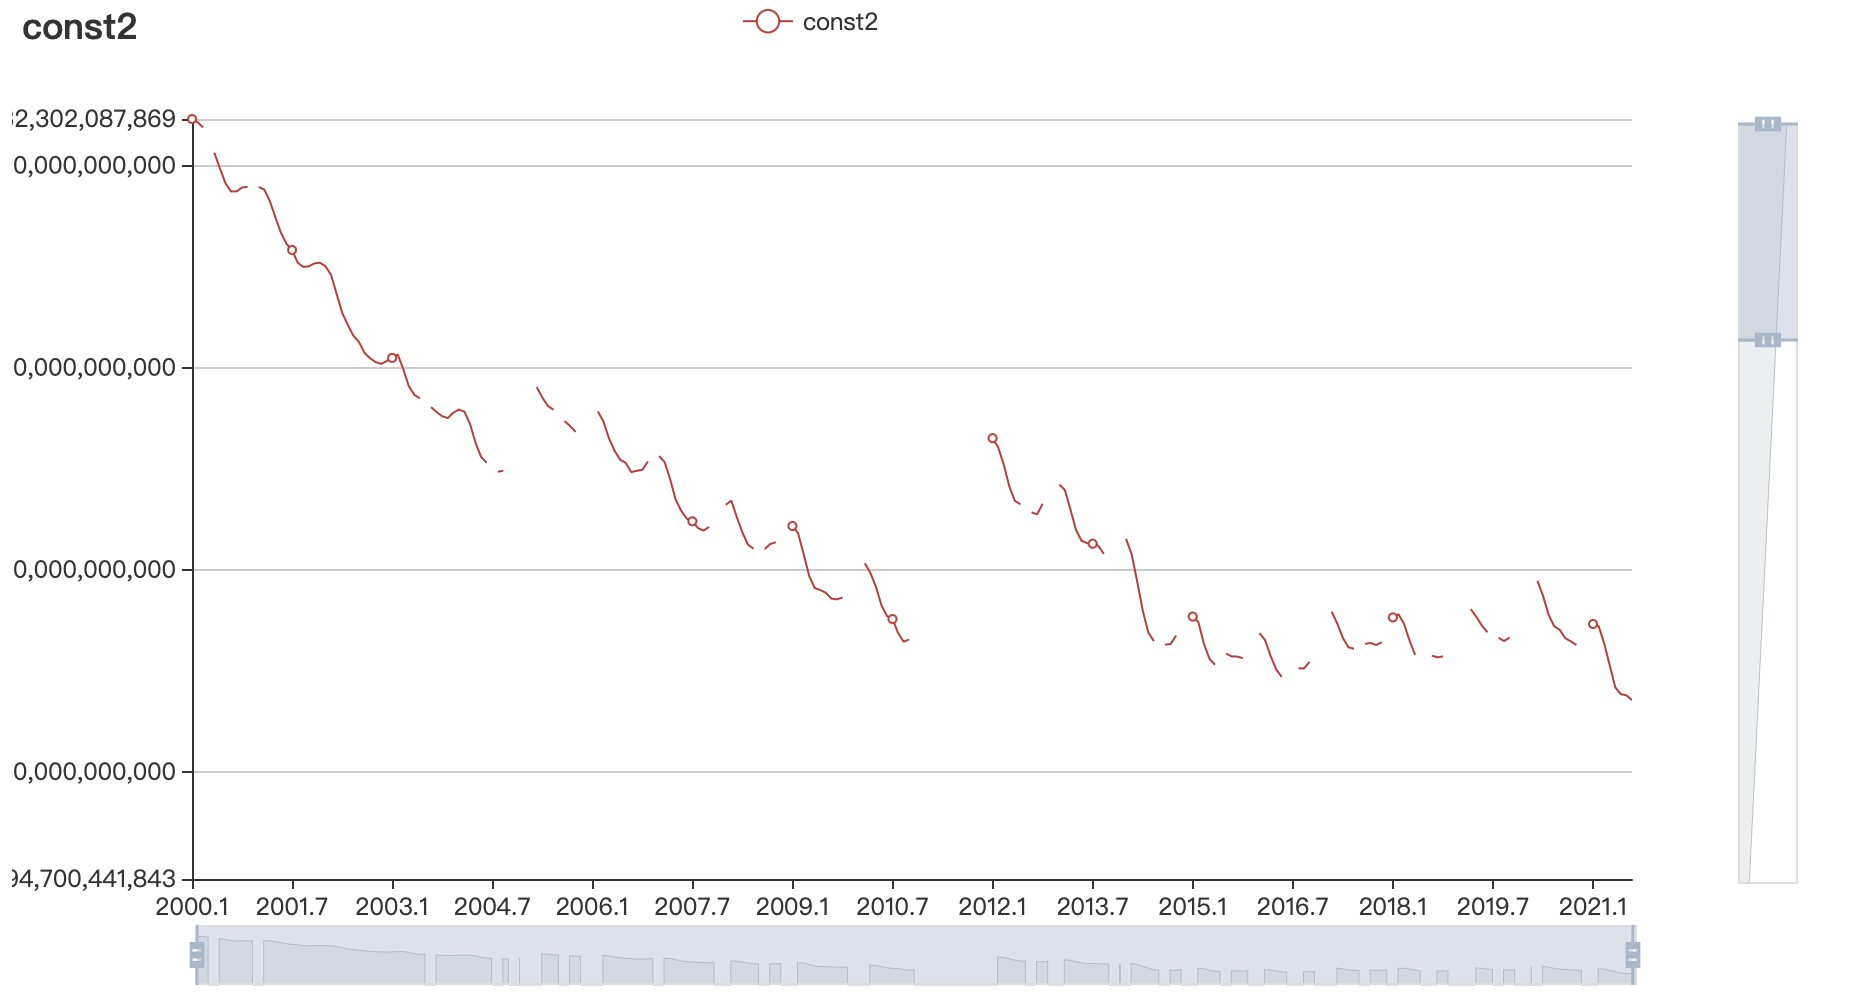
\includegraphics[width=10cm]{3.10 D_2 over time.jpg}

		\small \textit{Fig. 3.10 $D_2$ over time}
		\end{center}

		We can see that the variation of $D_1$ is periodical and small enough to be omitted. Therefore, we take the average of the previous $D_1$ and therefore the future functions are determined only by $D_2$. However, given the previous point on the graph, we can calculate the constant $D_2$ in each reduction step. 

		Assuming that $D_1$ remains the same as its average in the future and $D_2$ fits the first data point, we address the calculations in Jupyter Notebook and get Fig. 3.10 (the four approximate lines have different starting points).

		\begin{center}
		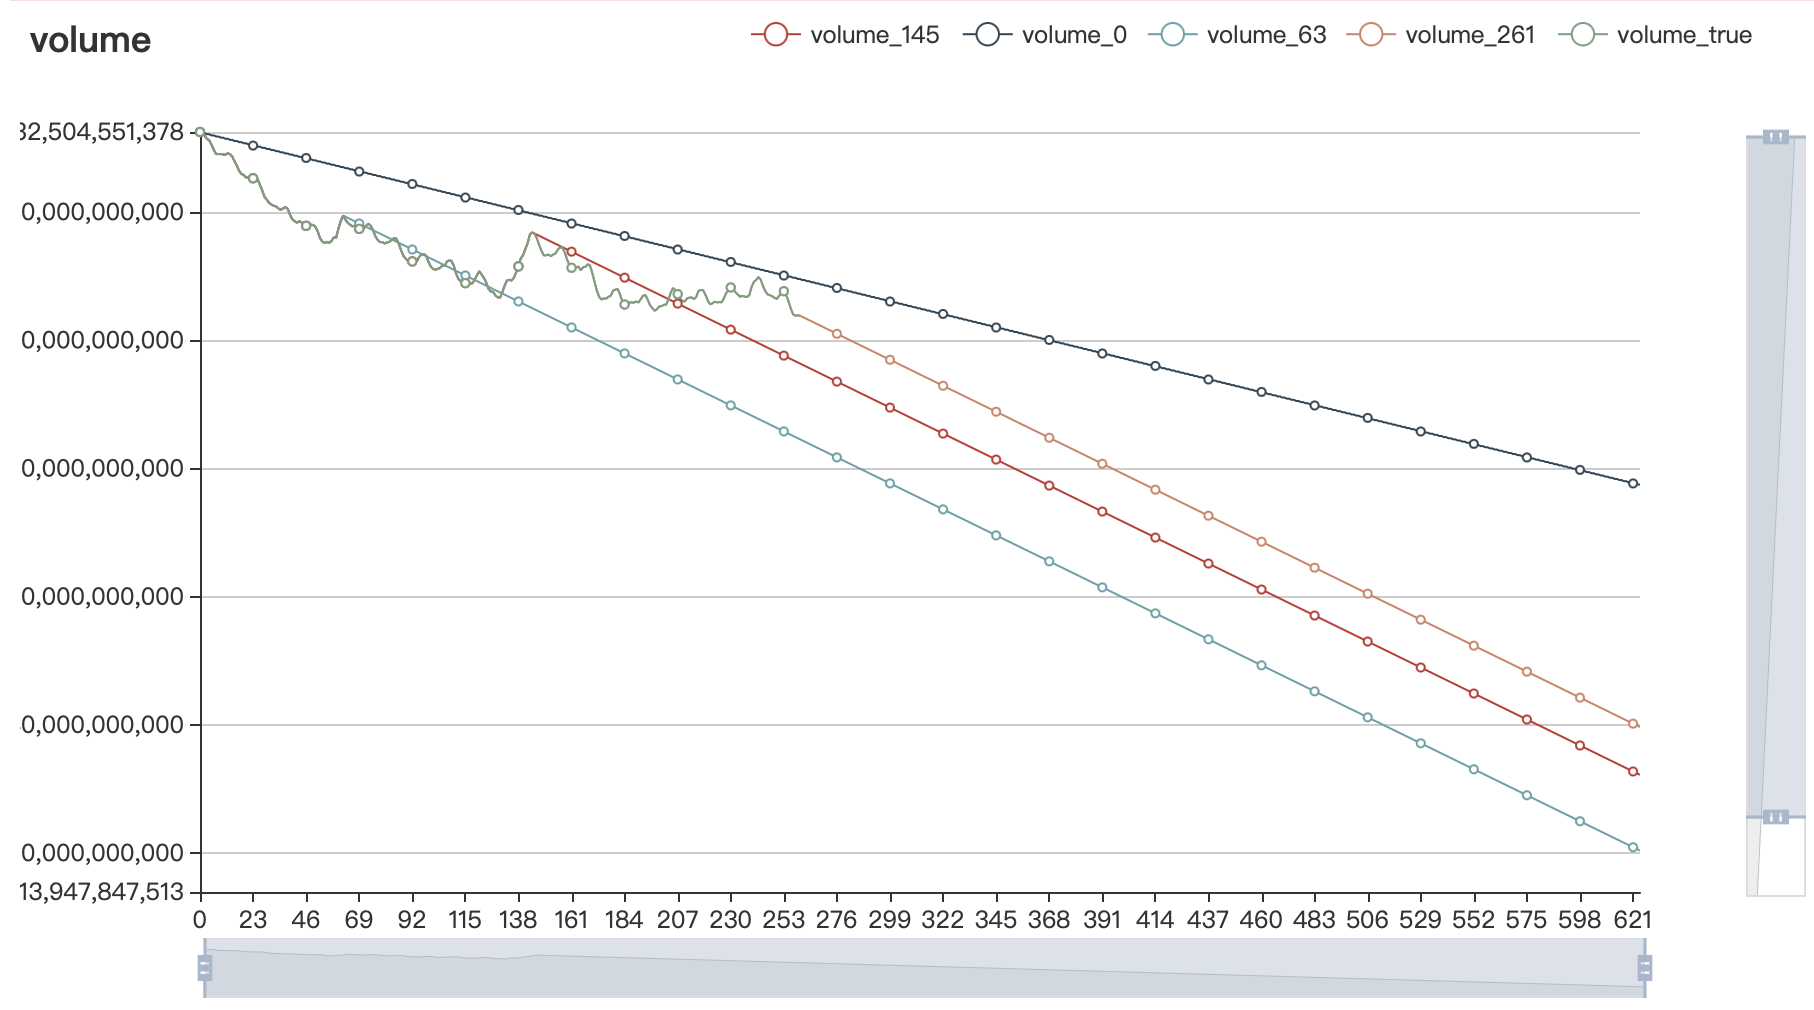
\includegraphics[width=10cm]{3.11 Results of Model 2.jpg}

		\small \textit{Fig. 3.11 Results of Model 2}
		\end{center}

		The results for Year 2025, 2030 and 2050 are as following:
		~\\
		\begin{center}
		\begin{tabular}{ccccc}
			\hline
			Year&Data Range&Mean Volume ($\rm{m^3}$)&Water Level (m)&Water Level (Inches)\\
			\hline
			2025&312-323&93714376236.411&309.58203&1015.6890\\
			2030&372-383&83137549287.743&293.02237&961.3595\\
			2050&612-623&40830241493.071&226.53862&743.2369\\
			\hline
		\end{tabular}
		\end{center}
		~\\

		These results are similar to Model 1 but less optimistic. Thus, we drew the conclusion that the most recent data lead to More accurate predictions when compared with the predictions in Model 1.

\newpage
\section{Wastewater Model}
	\subsection{Problem Overview}
		The water level of Lake Mead has great effects on the water use of Las Vegas citizens, and local governments has already introduced policies to reduce the use of water, especially in gardening. \cite{Actions Taken}

		Wastewater recycling is also an effective way to solve Lake Mead's problem and it may set a good example for all the countries to deal with their water pollution crisis. In this model, we mainly investigate on the plan of building sewage plants in the neighborhoods of Las Vegas. So the model is divided into three parts: considering the citizen's water-using condition, the location chosen to build the sewage plants and the function of sewage plants. Finally, we will give out a one-page report to show our plan and a serie of  policies to assist our plan.

	\subsection{Assumptions}
		\begin{itemize}
			\item \textbf{Every citizen produces the amount amount of wastewater every day.}

			\item \textbf{Every people is located in the center of his neighbohood.}
			
			As we assume that the neighborhood is some dots in the area, the position of citizens can be ignored.

			\item \textbf{Cost is not taken into consideration.}

			\item \textbf{All the population density is a same number.}
			
			All the citizens in Las Vegas is relatively averagely scattered, we can assume that the population density is the same.
		\end{itemize}

	\subsection{Factors}
		\begin{itemize}
			\item We took $d=\dfrac{\sum\limits_{i=1}^n(x_i\times d_i)}{\sum\limits_{i=1}^n(x_i)}$. $x_i$ refers to the number 
			of citizens in the neighbohoods while $d_i$ refers to the distance from the neighborhood to the chosen
			location.
			\item The distance from the chosen location to Las Vegas ( the place where treated water is discharged) is identified
			as $l$.
		\end{itemize}

	\subsection{Choose our location}
		\subsubsection{Every Day Water Usage}
			When we first investigate on choosing the location of sewage plants, the water using condition of the citizens in Las Vegas is the first to consider.
			We assume that the average water usage in this area is:

			$$V_{\text{used by human}}=\frac{annual\ per\ capita}{time}\times{n}$$

			So if x\% of the water comes from the upstream of the Colorado River and other tributaries while y\% comes from Lake Mead and (100-x-y)\% comes from the downstream part, we can get the following formulas:

			$$mean_{\text{used by human}}=\frac{{y\%}\times{annual\ per\ capita}}{time}\times{n}$$
			$$colorado_{\text{used by human}}=\frac{{x\%}\times{annual\ per\ capita}}{time}\times{n}$$

			These formulas can effectively describe the water used in the area.

		\subsubsection{Effectiveness}
			It's clear that we need to find an effective location, and the effectiveness of a sewage plant is related to the time it nedd to trasport the wastewater to the plant through pipes and its distance to Las Vegas Lake. When it comes to a parameter about the location, the effectiveness number $s$ should be as high as possible.

			We difine $s$ as

			$$s=\frac{k_1}{d}+\frac{k_2}{l},$$

			where $d$ refers to the distance from the location to the city center of Las Vegas and $l$ refers to the smallest distance from the location to Las Vegas Lake.

			For people need to transport the treated water to the Lake Mead area and the storage point, we can assume that the wastewater flow produced is continous, and because that gadget is not taken into consideration, we can ignore $k_1$ compared with $k_2$. So:

			$$s\approx\frac{k_2}{l}$$

			So we can infer that we need to build the sewage plants away from the Las Vegas Lake.

			\begin{center}
				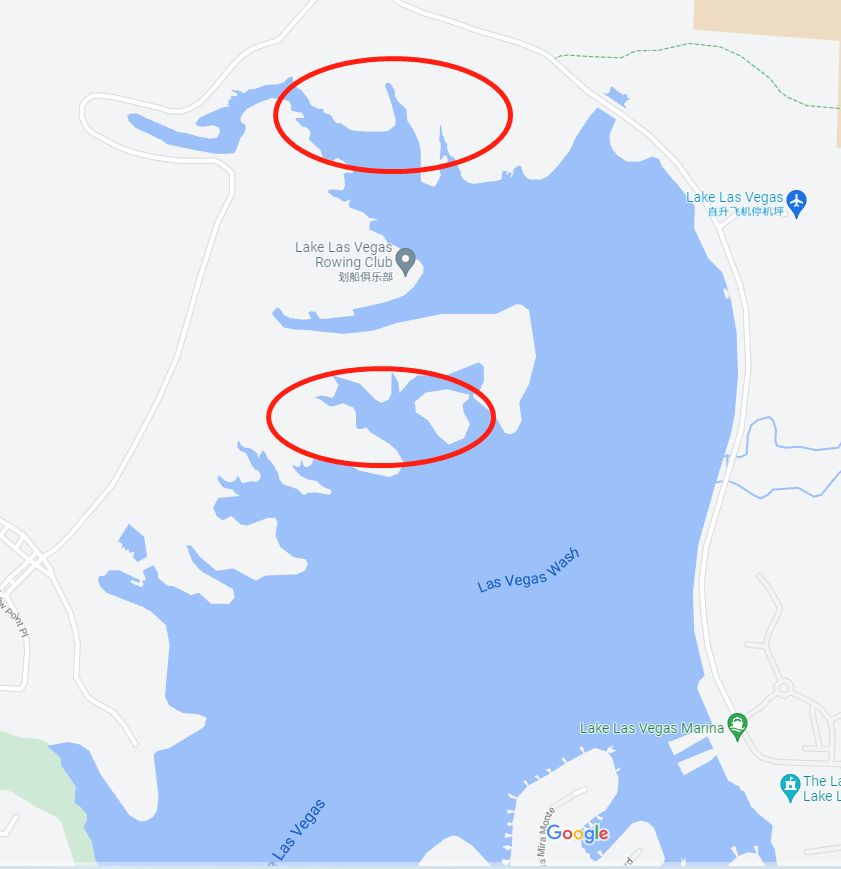
\includegraphics[width=10cm]{4.1 The Location for the Sewage Plant.png}
				
				\textit{Fig. 4.1 The Location for the Sewage Plant}
			\end{center}

			Fig. 4.1 is a map of Las Vegas Lake, and after close inspection, we pointed out some places that are suitable for building sewage plants.

\newpage
\section{Strengths and Weaknesses}
	\subsection{Strength}
		\begin{itemize}
			\item \textbf{Our model is high in universality.}
			
			Our model comes in cycles, so we can easily find the patterns in them and can it can be used in all kinds of  problems related with drought and water level.

			\item \textbf{We simplified the three-dimensional figure while making it fit the physical truth.}
			
			Although Lake Mead is an irregular shape, we simplify the lake into a regular shape without making it disobey the physical truth.

			\item \textbf{Our plan is easy to be carried out.}
			
			In our model, we put most of our attention on balancing between convenience for transport and convenience for citizens. This makes the model easier to be carried out.
		\end{itemize}

	\subsection{Weaknesses}
		\begin{itemize}
			\item \textbf{We lack accuracy in this model.}
			
			In this model, too many assumptions which are closely related to important factors are made in our model, this will make the model low in accuracy.
			
			\item \textbf{Too many averages are taken in our model.}
			
			To stablize the model, we make some averages in the process. This weakens the accuracy of our model.
		\end{itemize}

\newpage
\section{Final Report}
	Nowadays, with the negative impact of climate change, the fall of water level of Mead has become a serious problem for the people in Las Vegas and the nearby regions. So, we thought of an effective way to solve this problem----to recycle wastewater which flows in our sinks, toilets, and showers. This can fulfill the need for agriculture and everyday use.

	In our plan, there is a transporting process:
	We will first collect the wastewater into the pipes which will transport the wastewater to the sewage plant.
	After the water is processed and become drinkable, pipes will first transport water to fields where crops are grown to serve the agricultural purpose. 
	Then the water will be sent to Lake Mead which is now again a normal storage reservoir which will enable water usage of the people in Las Vegas as well as prepare for the coming drought.

	To realize our plan, several policies will be carried out:
	\begin{itemize}
		\item We will build one wastewater collector in three or four neighborhoods, this will make it easier for transportation.
		\item  If the amount of wastewater is over the amount the sewage plant can manage, we will either store the wastewater in the wastewater storage reservoir or emmit wastewater into the sea, using the power of nature.
		\item During drought period, we will strengthen the wastewater recycling treatment and will encourage people to use less water for the purpose of saving water.
	\end{itemize}

	This will require the Las Vegas government to set apartments to supervise the process. Also, sewage plants should also pay attention to the pollution it cause to the environment and it may be possible that they will treat the wastewater they produced to recycle wastewater. In addition, people should be reminded the fall of water level and the aggravation of the drought. Finally, the government could post a fine on the citizens for the emission of untreated watsewater.

	We believe that by carrying out this plan, Lake Mead will no longer suffer from the problem of water shortage and the agriculture as well as human well being will have a remarkable development.

\newpage
\thispagestyle{empty}
% \setcounter{page}{\wholepages}
\renewcommand\refname{Reference}
\clearpage
\addcontentsline{toc}{section}{References}
\tolerance=500
\begin{thebibliography}{100}
	\bibitem {Lake Mead} Wikipedia. Lake Mead.\\ https://en.wikipedia.org/wiki/Lake\_Mead

	\bibitem {Colorado River} Wikipedia. Colorado River.\\ https://en.wikipedia.org/wiki/Colorado\_River

	\bibitem {List of Dams} Wikipedia. List of dams in the Colorado River system.\\ https://en.wikipedia.org/wiki/List\_of\_dams\_in\_the\_Colorado\_River\_system

	\bibitem {Glen Canyon Dam} Wikipedia. Glen Canyon Dam.\\ https://en.wikipedia.org/wiki/Glen\_Canyon\_Dam

	\bibitem {Davis Dam} Wikipedia. Davis Dam.\\ https://en.wikipedia.org/wiki/Davis\_Dam

	\bibitem {Muddy River} Wikipedia. Muddy River (Nevada).\\ https://en.wikipedia.org/wiki/Muddy\_River\_(Nevada)

	\bibitem {Virgin River} Wikipedia. Virgin River.\\ https://en.wikipedia.org/wiki/Virgin\_River

	\bibitem {Vapor Pressure} Wikipedia. Vapor pressure.\\ https://en.wikipedia.org/wiki/Vapor\_pressure

	\bibitem {Water Level Data} U.S. Bureau of Reclamation. Archives of Daily Reservoir \& River Conditions for Lower Colorado Region.\\ https://www.usbr.gov/lc/region/g4000/levels\_archive.html

	\bibitem {Storage Data} National Parks Service. Storage capacity of Lake Mead.\\ https://www.nps.gov/lake/learn/nature/storage-capacity-of-lake-mead.htm.

	\bibitem {Temperature and Percipitation Data} Simulated historical climate \& weather data for Lake Mead National Recreation Area. meteoblue.\\ https://www.meteoblue.com/en/weather/historyclimate/climatemodelled/lake-mead-national-recreation-area\_united-states-of-america\_5506885

	\bibitem {Water Use in Las Vegas} UNLV COLA 101. Water Use in Las Vegas.\\ https://digitalscholarship.unlv.edu/cgi/viewcontent.cgi?article=1010\&context= cola\_ug\_research\_anthropology

	\bibitem {Actions Taken} Las Vegas Valley Water District. Drought and conservation measures.\\ https://www.lvvwd.com/conservation/measures/index.html

\end{thebibliography}
	
\end{document}